%%=============================================================================
%% Methodologie
%%=============================================================================

\chapter{\IfLanguageName{dutch}{Methodologie}{Methodology}}%
\label{ch:methodologie}

% Door de vergaarde kennis uit de literatuurstudie in hoofdstuk \ref{ch:stand-van-zaken} over de mogelijke noden van scholieren met dyslexie, de complexiteit van wetenschappelijke artikelen, de technieken voor MTS en ATS, en de bijhorende valkuilen bij taalverwerking met AI, kunnen onderzoeksmethoden worden toegepast om een antwoord te vinden op de onderzoeksvraag. 

Hiervoor moeten drie onderzoeksmethoden toegepast worden, met als hoofddoel het ontwikkelen van een prototype voor gepersonaliseerde ATS om wetenschappelijke artikelen te vereenvoudigen voor scholieren met dyslexie in de derde graad van het middelbaar onderwijs.

\section{Requirementsanalyse}
\label{sec:requirementsanalyse}

Om de ontwikkeling van het prototype zo gefocust te laten verlopen, moet het onderzoek stilstaan bij de toegepaste MTS en ATS technieken bij bestaande tools. Dit gebeurt door middel van een requirementsanalyse. Met een verkennend onderzoek en korte experimenten bouwt deze onderzoeksfase een Moscow-schema op met de nodige functionaliteiten voor ATS, met evenwaardige capabiliteiten als die van gepersonaliseerde MTS. De geteste toepassingen opgesomd in \ref{table:shortlist-tools} representeren de \textit{top-of-the-line} toepassingen voor (gepersonaliseerde) ATS. Zo omvat deze lijst zowel erkende toepassingen van de overheid, alsook toepassingen die leerkrachten of scholieren kunnen gebruiken om teksten te vereenvoudigen. Met deze onderzoeksmethode kan het onderzoek een antwoord geven op de volgende twee deelvragen van het onderzoek:

\begin{itemize}
	\item Welke functies ontbreken AI-toepassingen om geautomatiseerde tekstvereenvoudiging mogelijk te maken voor scholieren met dyslexie in de derde graad middelbaar onderwijs?
	\item Welke manuele methoden voor tekstvereenvoudiging komen niet in deze tools voor?
\end{itemize}

\medspace

De requirementsanalyse past de flowchart weergegeven in figuur \ref{img:flowchart-requirementsanalyse} toe. 

\begin{figure}[H]
	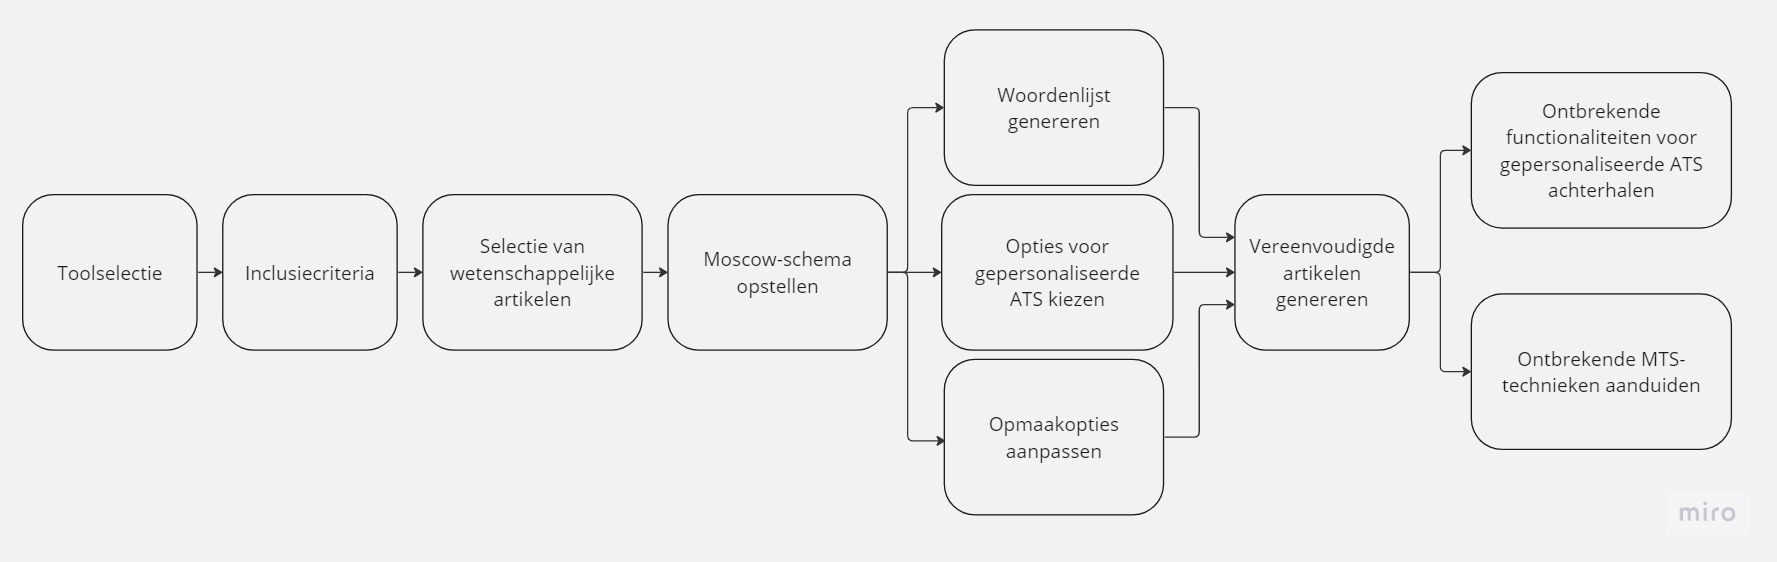
\includegraphics[width=\linewidth]{img/flowchart-requirementsanalyse.jpg}
	\caption{Het benodigde stappenplan bij de requirementanalyse.}
	\label{img:flowchart-requirementsanalyse}
\end{figure}

% TOOLSELECTIE 
Alvorens de requirementsanalyse van start kan gaan, moet het onderzoek een shortlist van tools kunnen selecteren. Zoals aangewezen in sectie \ref{sec:beschikbare-tools-en-taalmodellen}, beschikken scholen over vijf door de overheid erkende softwarepakketten, maar de requirementsanalyse betrekt enkel drie van deze vijf, omwille van hun prevalentie in het onderwijs en de functionaliteiten die de literatuurstudie eerder uitwees. Daarnaast kunnen online beschikbare tools ook scholieren met dyslexie ondersteunen bij het intensief lezen van wetenschappelijke artikelen met ATS, zoals bewezen in \textcite{Bingel2018}. De requirementsanalyse betrekt enkel tools met onderschreven tekstvereenvoudigingscapaciteiten en laat daarmee pure samenvattingstools erbuiten. Tabel \ref{table:shortlist-tools} geeft een overzicht weer van de tools waarvan het onderzoek experimenten op uitvoert.

\begin{center}
	\begin{table}[H]
		\begin{tabular}{ | m{6cm} | m{6cm} | } 
			\hline
			\textbf{Erkende software} & \textbf{Online beschikbare tools} \\
			\hline
			Sprintplus & Simplish \\
			Kurzweil3000 & SciSpace \\ 
			AlineaSuite & Rewordify\\
			& ChatGPT \\
			& Bing Chat\\
			\hline
		\end{tabular}
		\caption{Shortlist van uit te testen tools en toepassingen voor tekstvereenvoudiging.}
		\label{table:shortlist-tools}	
	\end{table}
\end{center}

% Inclusiecritera
Vervolgens moet het onderzoek criteria opstellen waarnaar de requirementsanalyse moet toetsen. Zo vormen de eerder benoemde MTS-technieken uit tabellen \ref{table:manual-simplification} en \ref{table:scientific-paper-struggles} de bouwstenen voor het valideren van de functionaliteiten bij tools op de shortlist. Met behulp van de criteria beschreven in tabel \ref{table:criteria-requirementsanalysis}, experimenteert deze onderzoeksfase met de toegelichte tools om de beschikbare en ontbrekende MTS-technieken te achterhalen, alsook of deze tools in staat zijn om wetenschappelijke artikelen te kunnen vereenvoudigen.

\begin{center}
	\begin{table}[H]
		\begin{tabular}{ | m{4cm} | m{11cm} | } 
			\hline
			\textbf{MTS-techniek} & \textbf{Functionaliteit} \\
			\hline
			Lexicale vereenvoudiging & Rekening houden met doelgroep buiten vakgebied door eenvoudigere synoniemen te schrijven \\
			& Woorden met minder lettergrepen gebruiken \\
			& Extra uitleg schrijven bij zinnen \\
			& Paragrafen herschrijven zodat ze eerst uitleg geven op een high-level niveau, vervolgens lagen van complexiteit toevoegen om de lezer te begeleiden \\
			& Woordenlijst aanmaken \\
			& Synoniemenlijst aanmaken \\
			& Idiomen vervangen door eenvoudigere synoniemen \\
			\hline
			Syntactische vereenvoudiging & Zinnen inkorten \\
			& Verwijswoorden aanpassen \\
			& Voorzetseluitdrukkingen \\
			& Samengestelde werkwoorden aanpassen \\
			& Actieve stem toepassen \\
			& Onregelmatige werkwoorden gebruiken \\
			\hline
			Structurele aanpassingen & Achtergrondkleur aanpassen \\
			& Woord- en karakterspatiering \\
			& Consistente lay-out \\
			& Duidelijk zichtbare koppenstructuur \\
			& Huidige positie benadrukken \\
			& Waarschuwingen geven omtrent formulieren en sessies \\
			& Inhoud visueel groeperen \\
			& Tekst herschrijven als tabel \\
			& Tekst herschrijven als opsomming \\
			\hline
		\end{tabular}
		\caption{Criteria waarop toepassingen worden afgetoetst in de requirementsanalyse.}
		\label{table:criteria-requirementsanalysis}	
	\end{table}
\end{center}

\medspace

% Wetenschappelijke artikelen kiezen
Als testmateriaal wordt er gebruik gemaakt van twee wetenschappelijke artikelen. Deze artikelen behandelen onderwerpen die interessant kunnen zijn voor scholieren in de derde graad van het middelbaar onderwijs, namelijk AI-surveillance in het artikel van \textcite{VanBrakel2022} en een economisch thema in het artikel van \textcite{Sleuwaegen2022}. Beide artikelen volgen de kenmerken van een wetenschappelijk artikel zoals beschreven in tabel \ref{table:scientific-paper-struggles}. Zo bevatten beide artikelen vakjarong en wetenschappelijke concepten in een compact formaat.

\medspace

% Opties voor gepersonaliseerde vereenvoudiging kiezen
Vervolgens benadert het onderzoek de verschillende tools om deze uit te testen, beginnend met de opties rond gepersonaliseerde vereenvoudiging te inspecteren. Alvorens de gepersonaliseerde tekstvereenvoudigingsmethoden aan bod komen, moeten de wetenschappelijke artikelen in de handen van de tool komen. Het uploaden van wetenschappelijke artikelen gebeurt bij SprintPlus, Kurzweil3000, AlineaSuite, Simplish en SciSpace met een PDF-upload, in tegenstelling tot Bing Chat en ChatGPT waarbij PDF-upload niet mogelijk is. Bij deze twee chatbots gebeurt de invoer met \textit{plain-text} als invoer of per link. De tekstinhoud uit de PDF extraheren gebeurt dan manueel en deze tekst dient daarna als invoer voor de chatbot. Beide chatbots krijgen dezelfde tekst voorafgaand van een prompt. Met vijf verschillende prompts kan het onderzoek de functionaliteit om lexicale, syntactische of structurele aanpassingen op een tekst achterhalen. Tabel \ref{table:tested-prompts-requirementsanalysis} vermeldt de toegepaste prompts. Tijdens het experiment krijgen de chatbots eerst een link naar het wetenschappelijk artikel mee, zoals aangegeven in figuur \ref{img:tryout-bing-ai}. Als de chatbot hier niet toe in staat is, dan krijgt de chatbot de tekstinhoud van het wetenschappelijk artikel als \textit{plain-text} mee. Vijf prompts, weergegeven in tabel \ref{table:tested-prompts-requirementsanalysis}, testen uit welke technieken van lexicale en syntactische vereenvoudiging of structurele aanpassingen deze chatbots kunnen uitvoeren.

\begin{center}
	\begin{table}[H]
		\begin{tabular}{ | m{2cm} | m{14cm} | } 
			\hline
			\textbf{Naam} & \textbf{Prompt} \\
			\hline
			P1 & Vereenvoudig deze tekst \\
			\hline
			P2 & Vereenvoudig deze tekst voor studenten (16-18 jaar) door moeilijke woorden te vervangen, vakjargon te schrappen, woorden langer dan 18 letters te vervangen, acroniemen voluit te schrijven, een woord slechts eenmaal door een synoniem te vervangen, korte uitleg te geven wanneer dat nodig is, en percentages te vervangen. \\
			\hline
			P3 & Vereenvoudig een tekst door deze op te delen in kortere zinnen van maximaal tien woorden. Verander voornaamwoorden als 'zij', 'hun' of 'hij' in namen. Vervang complexe zinsconstructies en voorzetselzinnen door eenvoudiger alternatieven, maar laat ze ongewijzigd als er geen eenvoudiger optie beschikbaar is. \\
			\hline
			P4 & Schrijf de tekst als opsomming. \\
			\hline
			P5 & Schrijf de tekst in tabelformaat. \\
			\hline
		\end{tabular}
		\caption{De toegepaste GPT-3-prompts in de requirementsanalyse.}
		\label{table:tested-prompts-requirementsanalysis}
	\end{table}
\end{center}

\begin{figure}[H]
	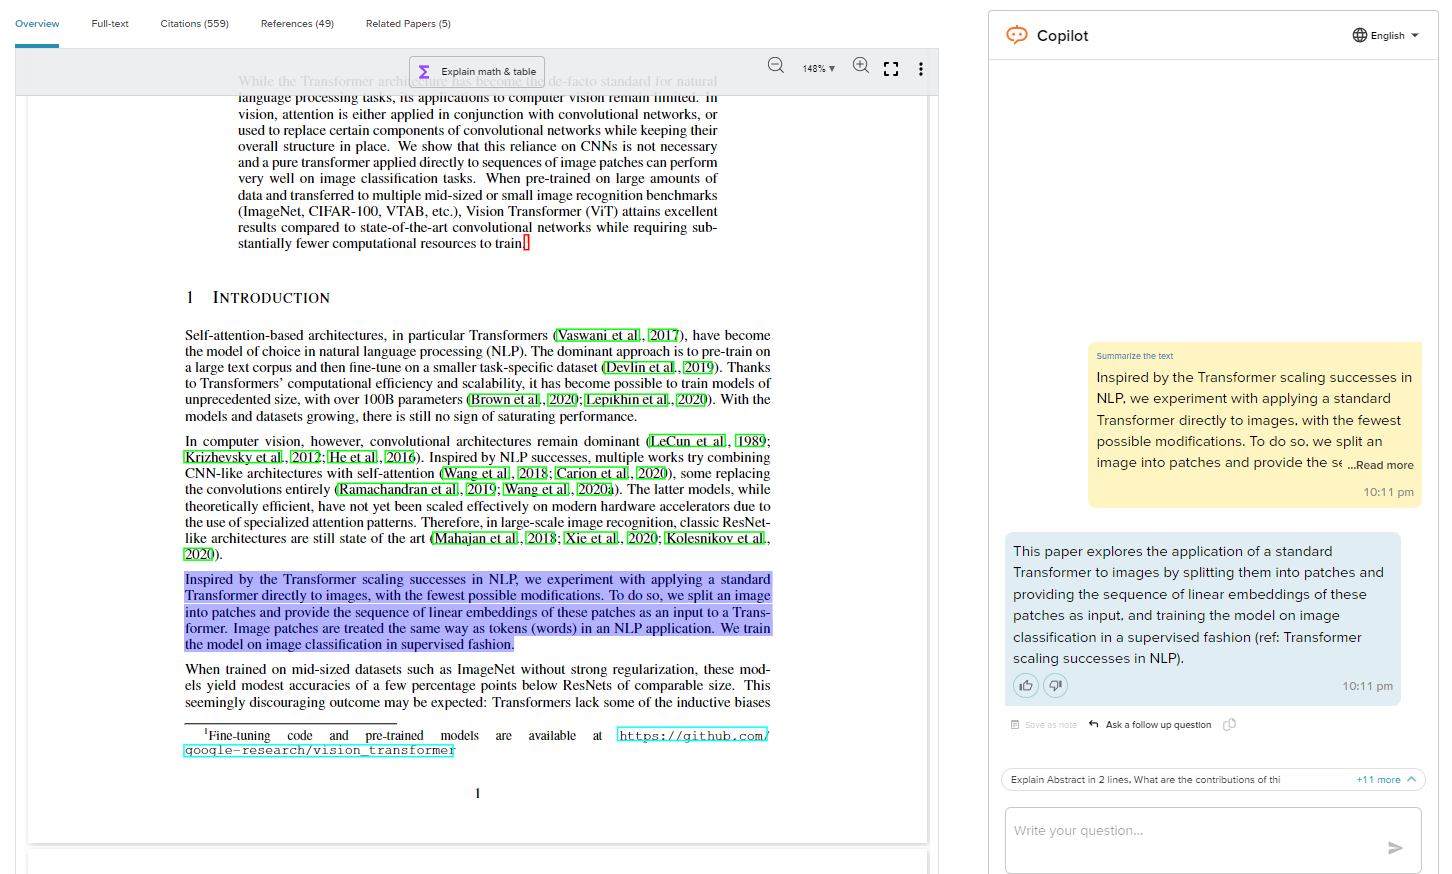
\includegraphics{img/typeset-example.png}
	\caption{Informatie opvragen van een wetenschappelijk artikel met SciSpace}
	\label{img:scispace-example}
\end{figure}

\begin{figure}[H]
	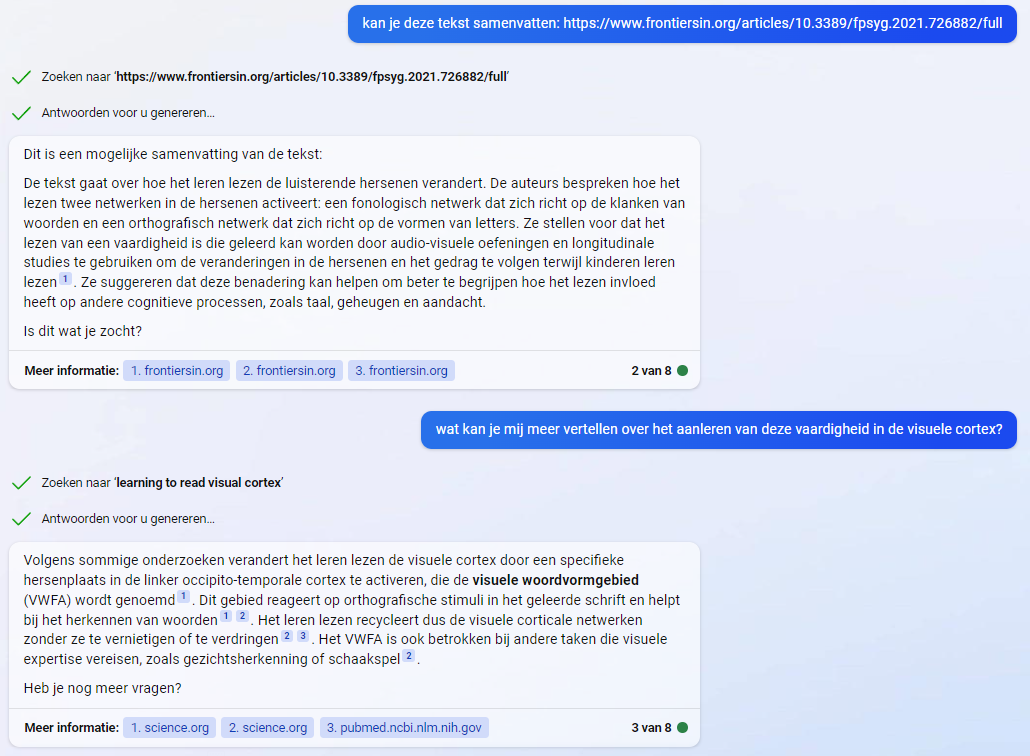
\includegraphics{img/bing-ai-chatbot-example.png}
	\caption{Tekstvereenvoudiging via de link van een wetenschappelijk artikel met Bing Chat}
	\label{img:tryout-bing-ai}
\end{figure}

\medspace

Woordenlijst genereren



Weergave of structurele opties aanpassen
De erkende software laat wel toe om lettertype -en grootte aan te passen. Deze fase komt bij de andere toepassingen echter niet aan bod.

\medspace

\begin{figure}[H]
	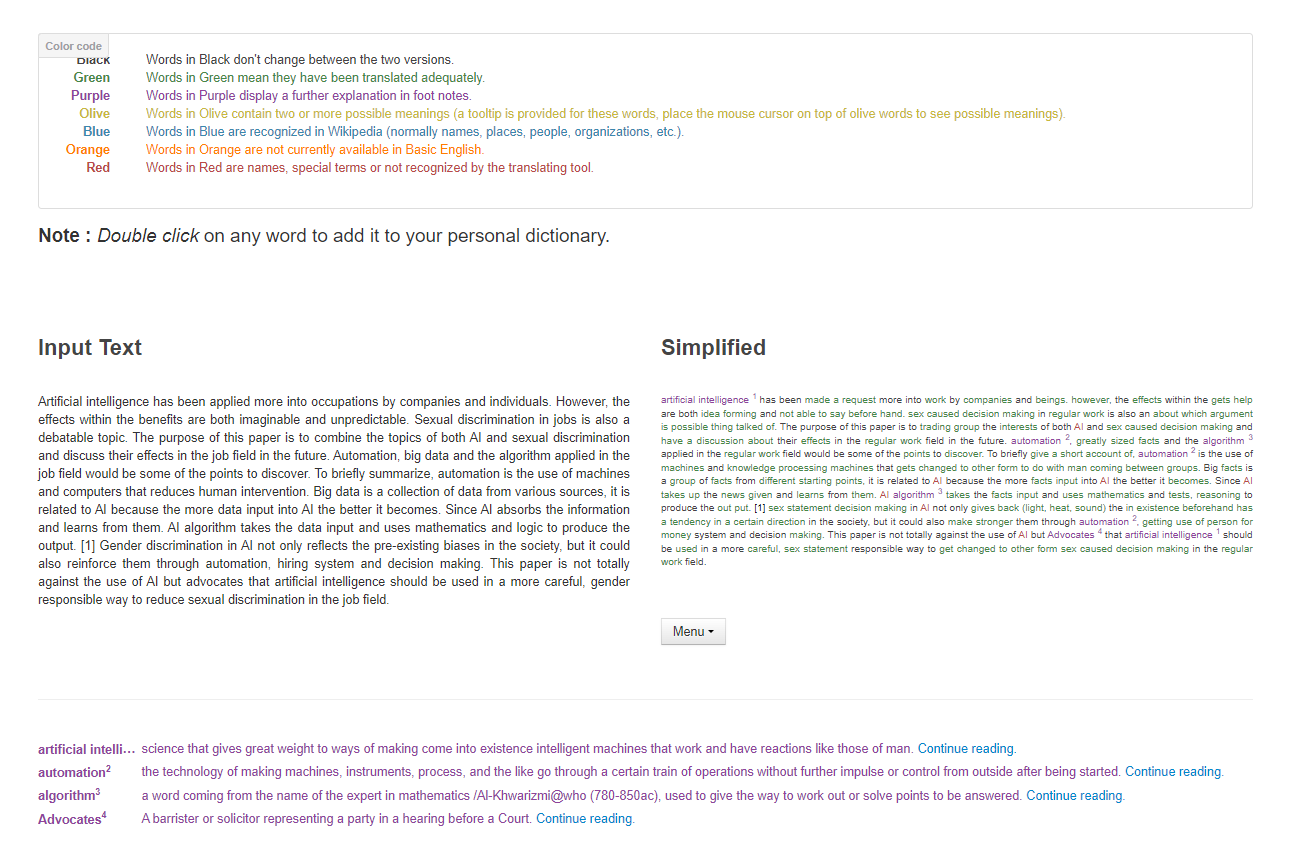
\includegraphics[width=\linewidth]{img/simplish-output.png}
	\caption{Illustratie van de tekstanalyse bij Simplish na een tekstvereenvoudiging.}
	\label{img:simplish-output}
\end{figure}

\begin{figure}[H]
	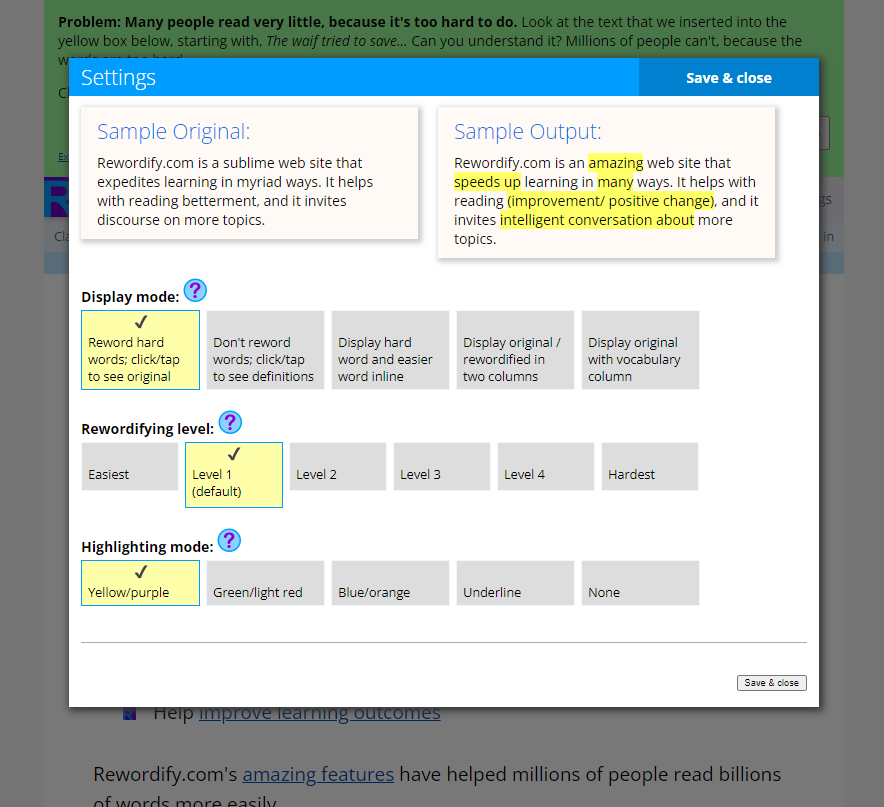
\includegraphics[width=\linewidth]{img/scholarcy-attempt.png}
	\caption{Illustratie van de tekstanalyse bij Rewordify.}
	\label{img:scholarcy}
\end{figure}

\medspace

Deze experimenten leiden tot een Moscow-schema dat fungeert als bouwsteen voor de ontwikkeling van het prototype voor gepersonaliseerde ATS van wetenschappelijke artikelen, specifiek op maat voor scholieren met dyslexie in de derde graad van het middelbaar onderwijs. Op basis van de afgetoetste criteria is de volgende Moscow-tabel, weergegeven in tabel \ref{img:moscow-table}, opgesteld.

\medspace

\begin{center}
	\begin{table}
	\begin{tabular}{ | m{4cm} | m{12cm} | } 
		\hline
		\textbf{MoSCoW-principe} & Functionaliteit \\
		\hline
		Must-have & Gepersonaliseerde vereenvoudiging aanbieden, waaronder lexicale en syntactische vereenvoudiging aanbieden, na het toevoegen van een respectievelijke API-sleutel. \\
		& Wetenschappelijke artikelen in PDF-vorm opladen. \\
		& Formaatwijzigingen toepassen aan de oorspronkelijke tekst. \\
		& Personaliseerbare toepassing: lettertype -en grootte aanpassen, tekstformaat aanpassen, achtergrondkleur aanpassen \\
		& Lokale opzet \\
		\hline
		Should-have & Glossary genereren na handmatige selectie van moeilijke woorden \\
		& Personaliseerbare PDF- of Worddocumentlay-out \\
		& Uitvoer als PDF of Word-bestand teruggeven. \\
		& Tekstanalyse voor en na de vereenvoudiging aanbieden. \\
		\hline
		Could-have & Glossary genereren na automatische selectie van moeilijke woorden \\
		\hline
		Wont-have & Beschikbaarheid tot de tool zonder Docker Desktop, in de vorm van online webtoepassing of browserextensie. \\
		& Beschikbaarheid tot de standaard- en gepersonaliseerde opties zonder API-sleutels \\
		\hline
	\end{tabular}
	\caption{Het Moscow-schema, opgebouwd door middel van de requirementsanalyse.}
	\label{img:moscow-table}
	\end{table}
\end{center}

\section{Vergelijkende studie}
\label{sec:vergelijkende-studie}

Teksten vereenvoudigen met ATS kan niet efficiënt verlopen zonder een taalmodel, maar een toepassing voor tekstvereenvoudiging binnen de casus van wetenschappelijke artikelen moet gebruik maken van een taalmodel die het meest aansluit op deze casus. Om het prototype af te stemmen op één taalmodel, vereist er een antwoord op de volgende vraag. 

\begin{itemize}
	\item Welk taalmodel of LLM is geschikt voor ATS van wetenschappelijke artikelen voor scholieren met dyslexie in de derde graad van het middelbaar onderwijs, met dezelfde of gelijkaardige kwaliteiten als gepersonaliseerde tekstvereenvoudiging met MTS?
\end{itemize}


Gezien de schaarse hoeveelheid aan gespecialiseerde taalmodellen, specifiek gericht op het vereenvoudigen van wetenschappelijke artikelen of taalmodellen met een personaliseerbaar karakter, beoordeelt de vergelijkende studie alle vermelde taalmodellen die speicifiek op ATS gericht zijn, beschreven in \ref{table:huggingface-models}. 

\begin{center}
	\begin{table}[H]
		\begin{tabular}{ | m{4cm} | m{12cm} | } 
			\hline
			\textbf{Verwijzing} & \textbf{Taalmodel} \\
			\hline
			T1 & Haining Scientific Abstract Simplification \\
			\hline
			T2 & BART-based Scientific Lay Summarizer \\
			\hline
			T3 & Keep It Simple\\
			\hline
			T4 & GPT-3 \\
			\hline
		\end{tabular}
		\caption{Gebruikte taalmodellen in de vergelijkende studie}
		\label{table:vergelijkende-studie-taalmodellen}
	\end{table}
\end{center}

\medspace

Zo vergelijkt deze onderzoeksfase de leesgraadsmetrieken van de oorspronkelijke wetenschappelijke artikelen zoals in \ref{sec:requirementsanalyse}, met referentieteksten vereenvoudigd via MTS en teksten vereenvoudigd met ATS. De referentieteksten zijn geschreven door twee leerkrachten binnen het vakgebied onderwijs, en twee scholieren van de derde graad in het middelbaar onderwijs zonder dyslexie. Deze vier personen baseren zich op vooraf meegekregen richtlijnen, toegelicht in de bijlage. Zinnen worden vereenvoudigd met ATS om zo het taalmodel met de beste ATS-capabiliteiten voor gepersonaliseerde ATS op te halen. Dit proces bestaat uit vijf fasen, weergegeven op het stappenplan in figuur \ref{img:flowchart-vergelijkende-studie-metrics}.

\begin{figure}
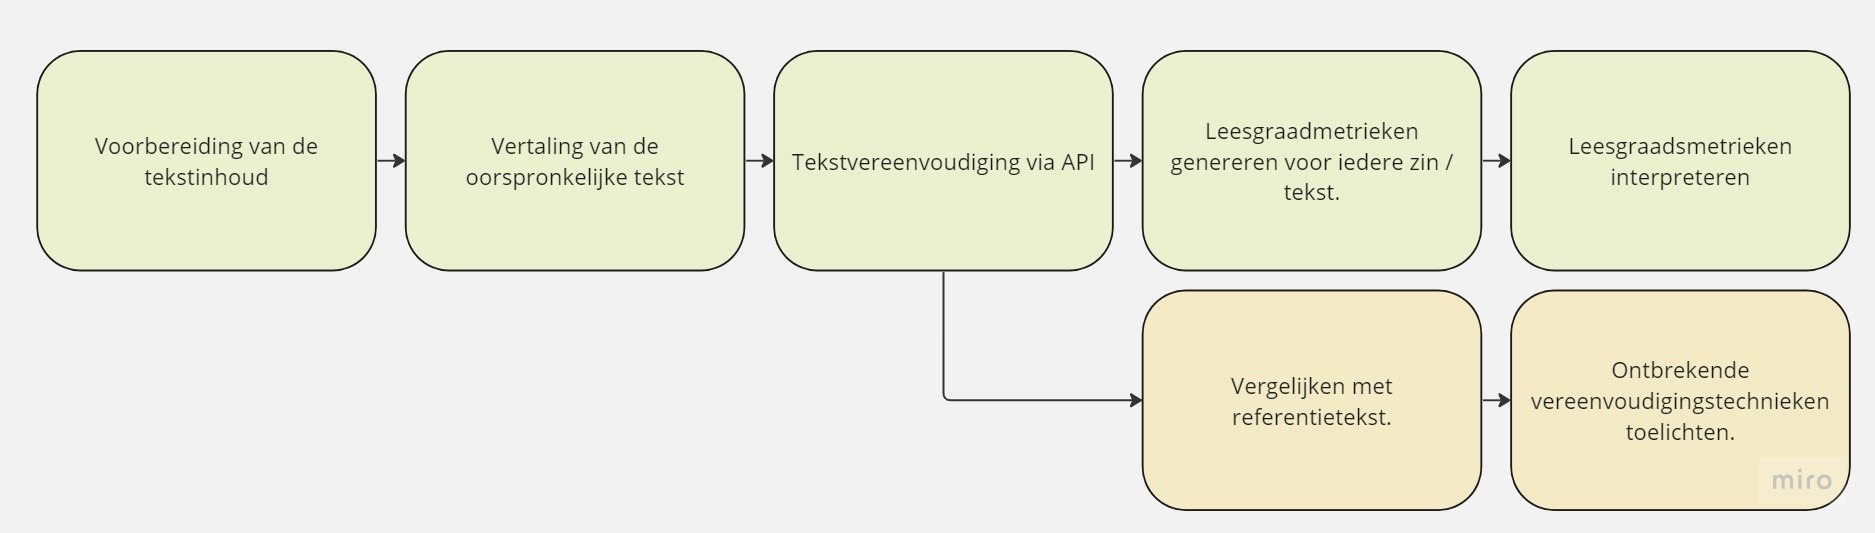
\includegraphics[width=\linewidth]{img/flowchart-vergelijkende-studie.jpg}
\caption{Het gevolgde stappenplan voor de vergelijkende studie.}
\label{img:flowchart-vergelijkende-studie-metrics}
\end{figure}

\medspace

% SCRIPT 1
Eerst volgt er een voorbereiding van de tekstinhoud. Allereerst haalt het script de inhoud van de map met wetenschappelijke artikelen op om deze vervolgens in een tekstbestand te plaatsen, zoals weergegeven in listing \ref{code:verg-studie-phase-1}. Dezelfde twee wetenschappelijke artikelen, namelijk \textcite{Sleuwaegen2022} en \textcite{VanBrakel2022}, komen in de vergelijkende studie aan bod.

\medspace

Vervolgens vertaalt het script de zinnen in het oorspronkelijk bestand naar het Engels. Het script, verwezen in script \ref{code:verg-studie-phase-2}, doorloopt alle tekstbestanden en vertaalt de tekstinhoud met de \textit{deep\_translator} Python-bibliotheek. Het resultaat van deze fase is een csv-bestand bestaande uit twee kolommen. Het resultaat van dit script is een csv-bestand met daarin twee kolommen, alle Nederlandstalige en alle vertaalde Engelstalige zinnen van één artikel. Een pipe-symbool dient als separator voor het csv-bestand.

\medspace

Na de vertaling vindt het aanspreken van het taalmodel plaats, weergegeven in code \ref{code:verg-studie-phase-3}. Vooraf vindt een tokenisatiefase plaats. De tokenisatie met Spacy gebruikt de embeddingsmodellen weergegeven in tabel \ref{table:wordembeddings-spacy}. Daarna vinden de API-calls plaats. API-calls in de \textit{scientific\_simplify}-functie naar HuggingFace of OpenAI regelen de taalverwerking. De request naar de HuggingFace API bestaat uit de parameters weergegeven in tabel \ref{table:huggingface-requests-parameters}. Deze taalmodellen moeten eerst beginnen en daarom krijgt de request een extra parameter, namelijk \textit{wait\_for\_model}. Verder past dit script geen extra parameters van de taalmodellen aan. Tabel \ref{table:tested-prompts} visualiseert de gebruikte prompts voor de testen bij het GPT-3 model. Zowel T1 als T4 maken gebruik van een \textit{nul-temperature} en een \textit{top-p} waarde van 90\% om zo een probabilisch vertrouwd antwoord te verkrijgen, net als om een hoge woordfrequentie te krijgen zoals aangegeven in \ref{table:gpt-3-parameters}. Bij T1 zijn deze parameters ingebakken. Nadien verwerken de taalmodellen iedere zin uit de tekst. Ten slotte beantwoordt de HuggingFace of GPT API in JSON-formaat, bevattende de vereenvoudigde versie van de opgegeven zin. T1, T2 en T3 vereenvoudigen de Engelstalige zinnen, in tegenstelling tot T4 en verwante prompts die de Nederlandstalige zinnen vereenvoudigen. Zoals aangehaald kunnen prompt-gebaseerde testen verschillende resultaten krijgen, afhankelijk van de gegeven input. Daarom benadert de vergelijkende studie drie verschillende prompts, gebaseerd op de tekstvereenvoudigingstechnieken beschreven in \ref{table:manual-simplification}. De tokenlengte kan een request doen falen. Daarom breekt het script de tekst per paragraaf op. 


\begin{center}
	\begin{table}[H]
		\begin{tabular}{ | m{4cm} | m{12cm} | } 
			\hline
			\textbf{Taal} & \textbf{Embeddingsmodel} \\
			\hline
			Nederlands & NL Core News Medium\footnote{https://github.com/explosion/spacy-models/releases/tag/nl\_core\_news\_md-3.5.0} \\ 
			\hline
			Engels & EN Core Web Medium\footnote{https://github.com/explosion/spacy-models/releases/tag/en\_core\_web\_md-3.5.0} \\
			\hline
		\end{tabular}
		\caption{Gebruikte SpaCy Word-embeddings}
		\label{table:wordembeddings-spacy}
	\end{table}
\end{center}

\begin{center}
	\begin{table}[H]
		\begin{tabular}{ | m{6cm} | m{6cm} | } 
			\hline
			\textbf{Naam parameter} & \textbf{Waarde} \\
			\hline
			Inputs & De oorspronkelijke zin. Enkel bij T1 komt 'simplify:' voor deze zin. \\
			\hline
			Max length & De lengte van de oorspronkelijke zin + 10 tokens. \\
			\hline
			Wait for model & Altijd ingesteld op \textit{True}. \\
			\hline
		\end{tabular}
		\caption{Meegegeven parameters bij HuggingFace-requests}
		\label{table:huggingface-requests-parameters}
	\end{table}
\end{center}

\medspace

\begin{center}
	\begin{table}[H]
		\begin{tabular}{ | m{2cm} | m{14cm} | } 
			\hline
			\textbf{Naam} & \textbf{Prompt} \\
			\hline
			P1 & Vereenvoudig deze tekst \\
			\hline
			P2 & Vereenvoudig deze tekst voor studenten (16-18 jaar) door moeilijke woorden te vervangen, vakjargon te schrappen, woorden langer dan 18 letters te vervangen, acroniemen voluit te schrijven, een woord slechts eenmaal door een synoniem te vervangen, korte uitleg te geven wanneer dat nodig is, en percentages te vervangen. \\
			\hline
			P3 & Vereenvoudig een tekst door deze op te delen in kortere zinnen van maximaal tien woorden. Verander voornaamwoorden als 'zij', 'hun' of 'hij' in namen. Vervang complexe zinsconstructies en voorzetselzinnen door eenvoudiger alternatieven, maar laat ze ongewijzigd als er geen eenvoudiger optie beschikbaar is. \\
			\hline
		\end{tabular}
		\caption{De GPT-3-prompts die in de vergelijkende studie aan bod komen.}
		\label{table:tested-prompts}
	\end{table}
\end{center}


% 
Vervolgens berekent het script in de vierde fase de benodigde leesgraadsmetrieken met de \textit{readability} Python-bibliotheek. Leesgraadsformules dienen, zoals aangegeven in \textcite{Nenkova2004}, als objectieve maatstaf bij deze vergelijkende studie. De bekomen leesgraadmetrieken ondergaan een vergelijking met elkaar en met die van een referentietekst. De vergelijking verloopt eerst objectief aan de hand van de leesgraadsmetrieken benoemd in tabel \ref{table:verg-studie-metrieken}. Code-blok \ref{code:verg-studie-phase-4} maakt een dataframe aan met de Pandas-bibliotheek. Het resultaat van dit script is een dataframe met alle leesbaarheidsmetrieken uit de \textit{readability}-library. Ten slotte eindigt het script door de dataframe op te slaan als CSV-bestand. Het visualiseren en interpreteren van de resultaten komt aan bod in de vijfde fase door middel van een Jupyter-notebook, waarbij de notebook Matplotlib gebruikt om resultaten te visualiseren.

\begin{center}
	\begin{table}[H]
		\begin{tabular}{ | m{8cm} | m{7cm} | } 
			\hline
			\textbf{Leesgraadsmetriek} & \textbf{Verwante vereenvoudigingstechniek }\\
			\hline
			FOG & Lexicale en syntactische vereenvoudiging \\
			\hline
			FRE & Lexicale en syntactische vereenvoudiging \\
			\hline
			Aantal woorden per zinnen & Syntactische vereenvoudiging \\
			\hline
			Aantal complexe woorden per zin volgens Dale Chall index & Lexicale vereenvoudiging \\
			\hline
			Aantal lange woorden per zin & Lexicale vereenvoudiging \\
			\hline
			Aantal gebruikte hulpwerkwoorden & Syntactische vereenvoudiging. \\
			\hline
			Aantal zinnen met een vervoeging van het werkwoord 'zijn' & Syntactische vereenvoudiging. \\
			\hline
		\end{tabular}
		\caption{De objectieve metrieken voor de vergelijking van de vereenvoudigde teksten met de oorspronkelijke tekst en de referentieteksten.}
		\label{table:verg-studie-metrieken}
	\end{table}
\end{center}

%
In tegenstelling tot de objectieve maatstaf kan de subjectieve evaluatie niet via leesgraadsmetrieken verlopen. De referentietekst dient hier als hulpmiddel om de referentietekst, ofwel het verwachte resultaat, te vergelijken met de vereenvoudigde tekst door een taalmodel. Naast leesgraadsmetrieken moeten de vereenvoudigde teksten eveneens de semantiek van de tekst kunnen behouden, alsook de volledige kern van de tekstinhoud nog steeds bijhouden. Zo moeten de referentieteksten capabel zijn om alle meegegeven vragen te beantwoorden. De aftoetsing gebeurt volgens de metrieken weergegeven in tabel \ref{table:verg-studie-reftekst-metrieken}.

\begin{center}
	\begin{table}[H]
		\begin{tabular}{ | m{7cm} | m{7cm} | } 
			\hline
			\textbf{Metriek} & \textbf{Verwante vereenvoudigingstechniek} \\
			\hline
			Inschatting van de doelgroep & Lexicale vereenvoudiging \\
			\hline
			Schrijven als tabelvorm of opsomming & Structurele aanpassing \\
			\hline
		\end{tabular}
	\caption{De subjectieve metrieken voor de vergelijking van de vereenvoudigde teksten door ATS met de referentieteksten.}
	\label{table:verg-studie-reftekst-metrieken}
	\end{table}
\end{center}

\section{Prototype voor tekstvereenvoudiging}

Met de benodigde functionaliteiten en de geschikte taalmodel voor gepersonaliseerde ATS, kan het onderzoek een volgende stap zetten richting de onderzoeksvraag. Deze sectie omschrijft de ontwikkeling van een prototype voor gepersonaliseerde tekstvereenvoudiging voor scholieren met dyslexie in de derde graad van het middelbaar onderwijs en geeft daarmee een antwoord op de volgende deelvraag: 

\begin{itemize}
	\item Hoe kan een intuïtieve en lokale webtoepassing worden ontwikkeld die zowel scholieren met dyslexie als docenten helpt bij het vereenvoudigen van wetenschappelijke artikelen met behoud van semantiek, jargon en zinsstructuren?
\end{itemize}

Allereerst moeten de gebruikte technologieën benadrukt worden. Eerdere onderzoeken maakten sporadisch gebruik van Python-technologieën en dit prototype volgt deze voorafgaande onderzoeken en vakliteratuur. Tabel \ref{table:technologies} geeft een breed overzicht van alle gebruikte programmeertalen. Hierop vult tabel \ref{table:python-libraries} aan door een overzicht te geven van alle gebruikte Python-libraries.

\begin{center}
	\begin{table}[H]
	\begin{tabular}{ | m{4cm} | m{12cm} | } 
		\hline
		\textbf{Technologie} & \textbf{Functionaliteit} \\
		\hline
		Python & De back-end van het prototype die API-calls en de NLP-functionaliteiten zoals PoS-tagging en lemmatizing verwerkt. \\
		\hline
		JavaScript & De toepassing gebruikersvriendelijker maken, personalisatie-opties voor de site doorvoeren en de functies gebouwd in Javascript dienen als alternatief op commandline instructies. \\
		\hline
		HTML en CSS & Het visuele uiterlijk van de website aanpassen naargelang de gekozen parameters van de eindgebruiker. \\
		\hline
		Jinja & Informatie uit de back-end (Python) doorgeven aan de front-end (JavaScript).  \\
		\hline
		Docker & Lokale uitrol van de webtoepassing. \\
		\hline
		Bash & Intuïtief script om de webtoepassing op te starten voor Linux en Mac-systemen. \\
		\hline
		Powershell & Intuïtief script om de webtoepassing op te starten op Windows-systemen. \\
		\hline
	\end{tabular}
	\caption{Gebruikte programmeertalen in het prototype voor tekstvereenvoudiging.}
	\label{table:technologies}
	\end{table}
\end{center}

\begin{center}
	\begin{table}[H]
	\begin{tabular}{ | m{4cm} | m{12cm} | } 
		\hline
		\textbf{Python-bibliotheek} & \textbf{Functionaliteit} \\
		\hline
		Flask					& Het framework van de webtoepassing. Deze combineert front-end en back-end en past binnen de scope van een prototype. \\ % later kan dan geopteerd worden voor een aparte front-end en back-end
		\hline
		PDFMiner 				& Tekstinhoud van PDF's inlezen. \\ 
		\hline
		EasyOCR					& PDF-pagina's inscannen als afbeelding in JPG-formaat om vervolgens de tekst te extraheren. \\
		\hline
		NumPy 					& De reshape-functie vereenvoudigt de manier om arrays van zinnen bij elkaar te plaatsen om zo een paragraaf te bekomen. \\
		\hline		
		Spacy 					& PoS-tagging en het lemmatiseren van woorden. \\
		\hline
		OpenAI					& GPT-3 API aanspreken. \\
		\hline
		Requests				& HuggingFace API aanspreken en informatie ophalen van een lexicale databank API. \\
		\hline
		BeautifulSoup			& HTML-content \textit{parsen} zodat de aangepaste inhoud van een leerkracht correct geformatteerd kan worden naar een PDF. \\
		\hline
	\end{tabular}
	\caption{Gebruikte Python-libraries en hun respectievelijke functie in het prototype.}
	\label{table:python-libraries}
	\end{table}
\end{center}

\medspace

De homepagina, weergegeven op figuur \ref{img:homepage}, biedt een kort overzicht van de twee algemene functionaliteiten, alsook instellingen waar gebruikers de webtoepassing kunnen aanpassen naargelang hun voorkeuren. Zoals aangeraden in \ref{ch:stand-van-zaken} door \textcite{Harvard2023}, moeten ontwikkelaars reking houden met de personalisering van de website. Deze functionaliteit gaat volgens hem vaak onopgemerkt en heeft nochtans een bewezen effect op het leesgedrag -en begrip van zowel mensen met als zonder dyslexie. De webtoepassing maakt gebruik van de standaardparameters, uitgewezen in \textcite{Rello2013a, Rello2013b}. Op een apart scherm kan de eindgebruiker de volgende elementen aanpassen naar hun toebehoren. Het prototype kan na aanpassing van de parameters eruit zien zoals weergegeven in figuur \ref{img:website-instellingen}. JavaScript maakt het mogelijk om deze parameters dynamisch en on-the-spot aan te passen. Na een aanpassing zal de back-end de sessievariabelen aanpassen naargelang de gekozen parameters, zodat de eindgebruiker niet per pagina deze parameters moet instellen. Voor dit prototype zijn er twee soorten eindgebruikers: leerkrachten die wetenschappelijke artikelen met ATS willen vereenvoudigen op maat van scholieren en de scholieren die dit zelf willen doen. Beide doelgroepen hebben hun eigen noden, maar toch een centraal doel voor ogen: het gepersonaliseerd vereenvoudigen van een wetenschappelijk artikel.


\begin{center}
	\begin{figure}[H]
		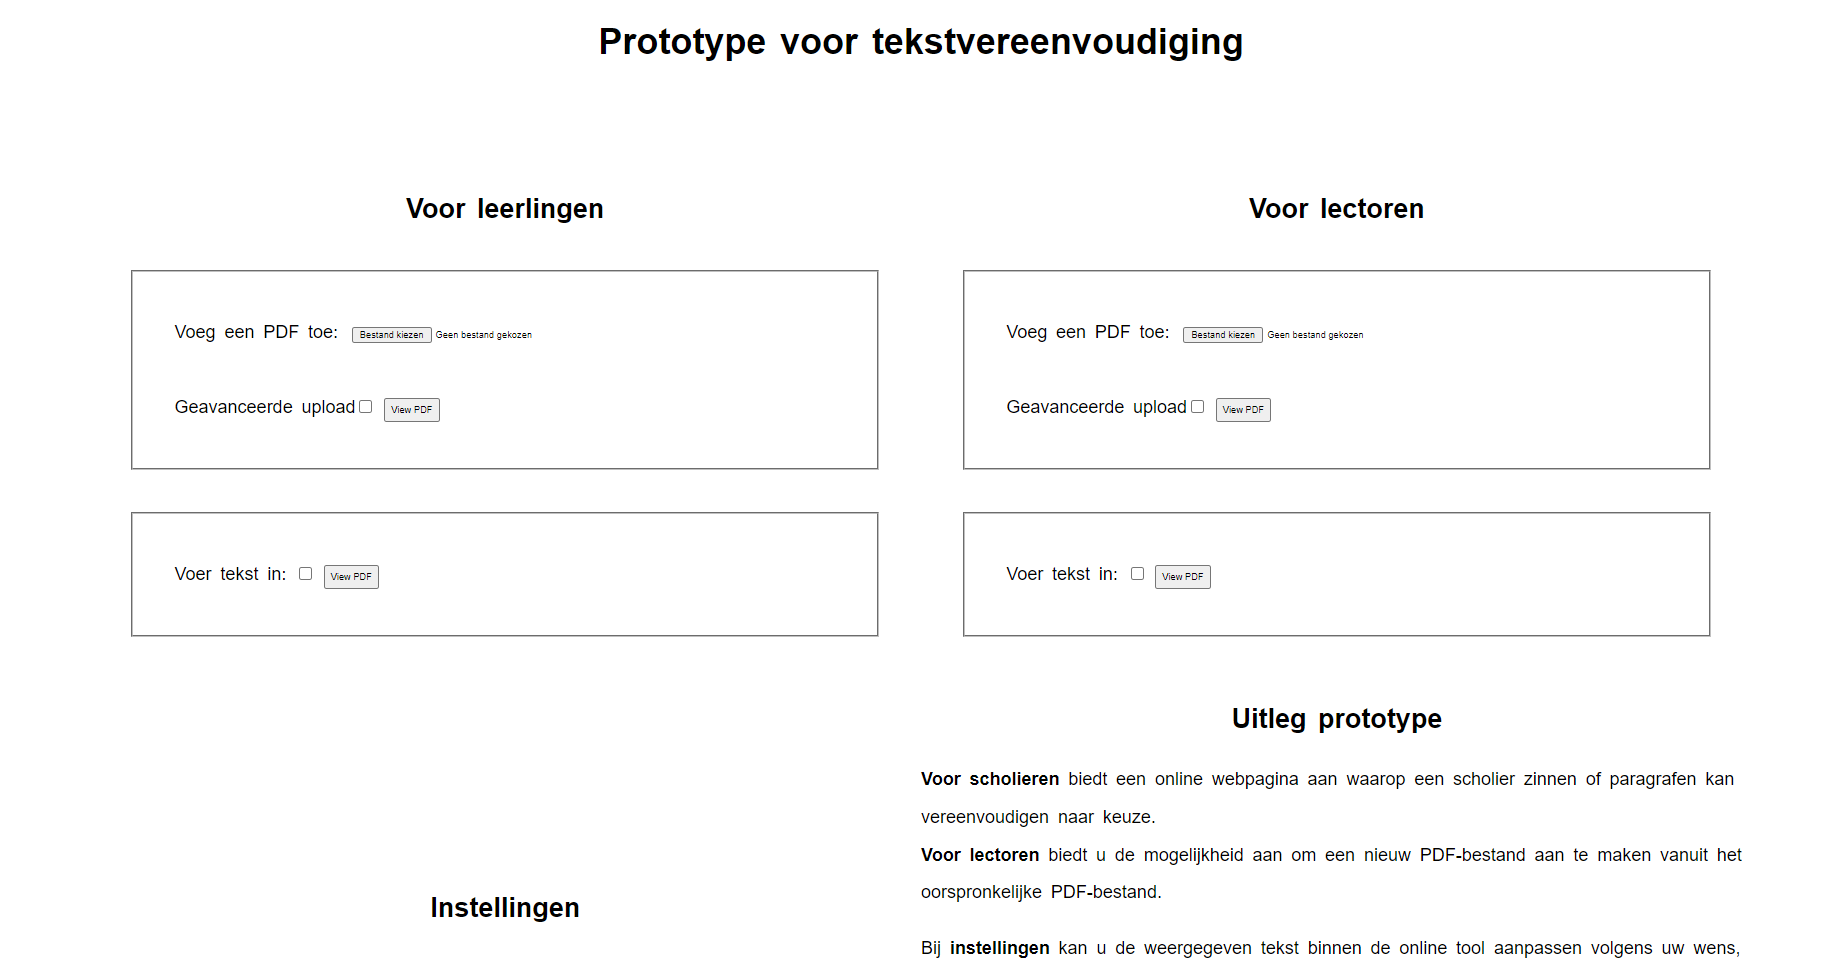
\includegraphics[width=\linewidth]{img/proto-homescreen.png}
		\caption{Een mogelijke weergaven van de homepagina.}		
		\label{img:homepage}
	\end{figure}
\end{center}

\begin{center}
	\begin{figure}[H]
		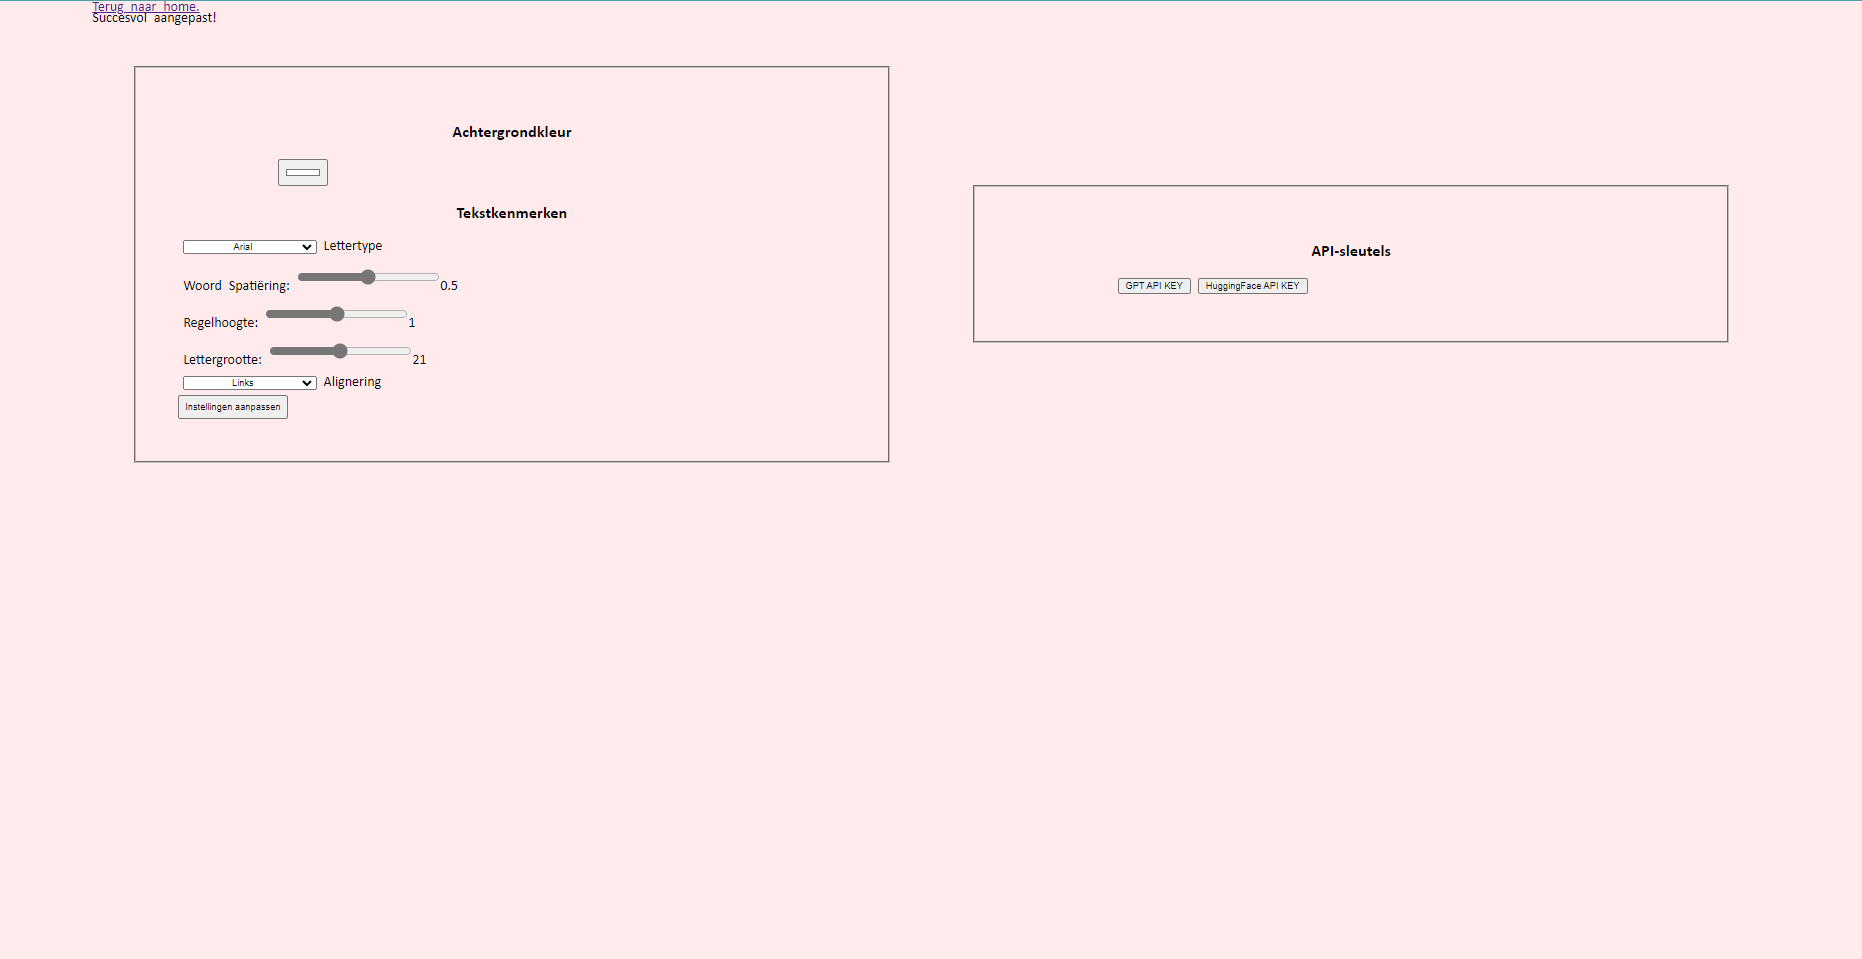
\includegraphics[width=\linewidth]{img/website-instellingen.png}
		\caption{Voorbeeldweergave van de instellingenpagina.}
		\label{img:website-instellingen}
	\end{figure}
\end{center}

De invoer van een wetenschappelijk artikel gebeurt voor beide doelgroepen op identieke wijze. De gebruiker kan een PDF of een stuk \textit{plain-text} ingeven als invoer van het wetenschappelijk artikel. Eindgebruikers kunnen met het prototype wetenschappelijke artikelen op één van twee manieren inladen: \textit{plaintext} of via een PDF-bestand. PDF's worden tijdelijk \textit{in-memory} opgeslaan. Daarmee kan het systeem niet na lange duur overbelast raken. Het prototype past eenzelfde functie toe om wetenschappelijke artikelen in te lezen voor de twee verschillende doelgroepen. Vooraf controleert de Flask-applicatie het type invoer. Vervolgens spreekt de Flask back-end de Reader-klasse aan die de tekst verder zal formatteren tot een bruikbaar formaat voor de webtoepassing. PDF extractors, waaronder PDFMiner, kunnen tekstinhoud verliezen tijdens het extraheren zoals eerder aangewezen in tabel \ref{sec:requirementsanalyse}. Als vangnet biedt het prototype een tweede optie aan waarbij de PDF-pagina's als afbeelding worden opgeslaan. Er wordt rekening gehouden met de splitsing tussen normale en geavanceerde upload. Deze twee methoden zijn terug te vinden in de Reader-klasse\footnote{https://github.com/Dyashen/text-simplification-tool/blob/main/web-app/Reader.py} ofwel bijlage \ref{code:reader-klasse}.

\begin{enumerate}
	\item PDFMiner itereert doorheen de PDF en extraheert vervolgens de tekst op iedere pagina. Deze methode resulteert in een string-object.
	\item De Python-bibliotheek EasyOCR voorziet een eenduidige en ontwikkelaarsvriendelijke manier om PDF-pagina's op te slaan als JPG of PNG. Tesserat biedt een even eenduidige oplossing aan, maar vergt meer configuraties en daarmee vergroot de omvang van de Docker-container. Vervolgens worden de afbeeldingen per text-chunk ingelezen en nadien opgeslaan. Het gebruik van deze alternatieve methode kan de omvang van de Docker-container vergroten. Om dit te voorkomen, verwijdert het prototype afbeeldingen nadat deze de tekstinhoud hebben geëxtraheerd en opgeslaan om zo ruimte te besparen. Net zoals bij de eerste methode resulteert deze methode in een string-object.
\end{enumerate}

De eerste fase van het prototype slaat de tekstinhoud op in meerdere arrays die zinnen voorstellen. Zoals aangegeven in \ref{code:reader-klasse}, staat de standaardparameter voor het aantal zinnen per paragraaf ingesteld op vijf zinnen, maar kunnen gebruikers aanpassen via het HTML-formulier bij de instellingen. Om de PoS-tag bij het respectievelijke woord bij te houden, maakt het prototype gebruik van een \textit{key-value pair} datastructuur. Zo verwijst de sleutel naar het woord in een zin; de waarde verwijst naar de PoS-tag die aan het woord toebehoord. Het prototype is enkel ontworpen voor Nederlandstalige en Engelstalige wetenschappelijke artikelen. Daarmee laadt het enkel twee embeddingsmodellen van Spacy op, zoals vermeldt in tabel \ref{table:wordembeddings-spacy}. Hardcoderen is uit den boze en daarom maakt het prototype gebruik van een \textit{dictionary} die de naam van deze embeddingsmodellen bijhoudt, zoals aangegeven in \ref{code:reader-klasse}. Zo is het systeem en hoeft er enkel een taalherkenning plaats te vinden. Fouttolerantie aanbieden gebeurt in de vorm van een standaardtaal in de dictionary, namelijk het Nederlands, of door vooraf de gebruiker te vragen in welke taal de opgelade tekst staat via een HTML-formulier.

% Deze transformatie bevoordeelt het proces om vervolgens de teksten per zin op de webpagina uit te printen. Bovendien is het manipuleren van het aantal zinnen per paragraaf een bewezen effect om de leesbaarheid van een tekst te verbeteren. 


\subsection{Tool voor leerkrachten}

In de vorm van een HTML-formulier kunnen leerkrachten gepersonaliseerde ATS met dit prototype waarmaken. Op de overzichtspagina kunnen leerkrachten beschikken over de functionaliteiten, weergegeven in tabel \ref{table:functionaliteiten-leerkrachten}. Het HTML-formulier omvat alle benodigde tekstvereenvoudigingstechnieken op lexicaal en syntactisch niveau die \ref{table:criteria-requirementsanalysis} verder uitwees. 

\begin{center}
	\begin{table}
		\begin{tabular}{ | m{7cm} | m{7cm} } 
			\hline
			\textbf{Functionaliteit} & Gebruikte JS/Python-techniek \\
			\hline
			Specifieke meegeven per paragraaf & Naast een optie om voor het hele document één prompt te gebruiken, voegt het prototype ook een optie toe om. Hiervoor past de web-inhoud een key-value structuur toe. \\
			\hline
			Opties voor gepersonaliseerde ATS aangeven. & Met behulp van een HTML-formulier kunnen leerkrachten checkboxes afvinken waaraan de gegenereerde tekst moet voldoen. Deze verschillende opties zijn terug te vinden in \ref{table:criteria-requirementsanalysis}. \\
			\hline
			Werkwoorden, bijvoeglijke en zelfstandige naamwoorden markeren & Front-end aanpassing met eventlistener. De tekstkleur van het aangeduide type woorden verandert naar het gekozen kleur. \\
			\hline
			Zinnen verwijderen & Front-end filter aangesproken door een \textit{eventlistener}. \\
			\hline
			Woord toevoegen aan woordenlijst & Een eventlistener handelt de functionaliteit af door de woorden en hun zin van voorkomen tijdelijk op te slaan in een storage. Het formulier houdt dit bij en geeft het vervolgens mee bij het indienen. Deze woorden en hun respectievelijke zin van voorkomen dienen om de woordenlijst op te vullen in het gegenereerde PDF of Word-bestand.\\ 
			\hline
			API-sleutel en sessieherkenning & Detectie met JS of een sessievariabele bestaat.
			\hline 
		\end{tabular}
	\caption{Alle beschikbare functionaliteiten in }
	\label{table:functionaliteiten-leerkrachten}
	\end{table}
\end{center}



\medspace

Om afwijkende resultaten op een GPT-prompt te vermijden, wordt de temperature op nul geplaatst en de \textit{top\_p} waarde wordt ingeschat op 80\%. SpaCy wordt gebruikt om woordkenmerken zoals de PoS-tag op te halen, maar het systeem is vatbaar voor het niet kunnen vinden van afwisselende en meertalige woordenschat. Een mogelijke oplossing is om de taal te veranderen naar Engels of Frans, of een aangepast taalherkenningsmodel te gebruiken. Een andere optie is om de tekst voor te verwerken om de Nederlandse en Engelse woorden te scheiden voordat ze worden verwerkt met SpaCy. Adjectieven uit de tekst verwijderen is mogelijk zonder taalmodel. Aangezien alle woorden gekoppeld worden aan een PoS-tag, is het eenvoudig om de woorden gelinkt aan de span-tag van de adjectieven uit te filteren.

\medspace

De eenduidige HTML-structuur van online woordenboeken maken het mogelijk om gratis en eenvoudig de definities van woorden op te halen. Zo is het mogelijk om annotaties op te halen zoals aangewezen in het onderzoek van \textcite{Bulte2018}. Met behulp van Requests en BeautifulSoup is het mogelijk om lijsten met definities te scrapen van deze sites. De stam van het gemarkeerde woord wordt opgehaald en vervolgens meegegeven als zoekopdracht. De bron wordt samen met het resultaat aan de eindgebruiker getoond. 

\subsubsection{Tekstvereenvoudiging}

Het prototype gebruikt een taalmodel van \textit{HuggingFace} voor extraherende samenvattingen en zowel gratis taalmodellen van \textit{HuggingFace} als het GPT-3 taalmodel voor abstraherende samenvattingen. Het model kan parameters, zoals maximale lengte van de gegenereerde tekst, ontvangen en biedt zowel gepersonaliseerde als niet-gepersonaliseerde vereenvoudiging. Het gebruik van \textit{HuggingFace} vereist een internetverbinding en kan geen extra trainingsdata bevatten. De opstarttijd voor alle \textit{HuggingFace}-taalmodellen wordt bij de start van de applicatie afgehandeld door middel van een extra parameter de request. Sleutels worden standaard bijgehouden in env-bestanden. Via de webtoepassing kan een gebruiker deze sleutel aanpassen. Binnen een lokale omgeving is dit in orde, al moeten ontwikkelaars rekening houden met beveiligingsmaatregelen wanneer een dergelijke tool wordt uitgerold. Het merendeel van de gebruikte taalmodellen is Engelstalig of is nadrukkelijk getraind op basis van Engelstalige datasets. De ingegeven tekst wordt eerst vertaald naar het Engels om zo de kans op een accurate vereenvoudiging te verhogen. Voor de vertaling wordt de Google Translate Python-package gebruikt. Deze is minder accuraat vergeleken met DeepL, maar biedt een gratis beschikbaar en aanvaardbaar alternatief aan. Factoren zoals topic diversity en semantische redundantie moeten overwogen worden bij het kiezen van een taalmodel voor extraherend samenvatten. Lange documenten samenvatten kan zoals aangeduid in literatuurstudie door extraherende samenvatting, gevolgd door abstraherende samenvatting om de tekst coherent te doen blijken. Eerder werd er gekozen om de voltekst per paragraaf bij te houden. Uit iedere paragraaf wordt een ideaal aantal zinnen gemarkeerd om nadien geparafraseerd te worden door GPT-3 of een \textit{HuggingFace} taalmodel, afhankelijk van de keuze van de eindgebruiker.


% TODO GPT-3

Bij de inference API van T1 moet er expliciet worden aangegeven om welke transformatie dit gaat door kernwoorden zoals 'simplify:'.

\medspace

De Creator-klasse bouwt PDF's en docx-documenten op volgens de meegegeven personalisatie en maakt gebruik van Pandoc via Python. Pandoc voert een tweestapsbeweging uit, waarbij het eerst plain-text naar een Markdown-formaat omzet en vervolgens het Markdown-bestand naar een PDF of Word-document converteert. Hiervoor is er eerst een YAML-header nodig. Deze header bevat de titel, standaardlettertype en lettertype voor de titel, de datum, het type document, de marge-instelling, de standaardlettergrootte, woord-spatiëring en de instelling voor de regeleinde. Het script voegt de meegekregen instellingen toe aan de LaTeX YAML-header. Om de woordenlijst in een PDF te maken, bouwt het script eerst een dictionary op met de positie als key en als values het woord, de PoS-tag en de opgehaalde gepersonaliseerde betekenis. De key is hier niet het woord, want het prototype moet rekening houden met homoniemen. Als de dictionary leeg is, dan wordt dit deel overgeslaan. De vereenvoudigde tekst is eveneens in een dictionary-structuur opgeslaan. De keys stellen titels voor en worden uitgeprint voorafgegaan door twee hekje-symbolen. Tussen de titels worden breaklines toegevoegd, gevolgd door de tekst die bij de titel bijhoort. Indien gekozen werd voor een opsomming, dan wordt er gebruik gemaakt van een geneste for-lus waarbij iedere zin wordt voorafgegaan aan een asterisk-symbool. De woordenlijst en vereenvoudigde tekst worden naar hetzelfde Markdown-bestand uitgeschreven. Als invoer wordt het pad naar opgevulde Markdown-bestand meegegeven. De uitvoer is het pad waarnaar het PDF- of DOCX-bestand moet worden opgeslaan. Vervolgens zet Pandoc het Markdown-bestand om naar een PDF-bestand gebouwd met de XeLateX engine of een Word-bestand op basis van meegekregen binaries. Pandoc Flask kan enkel één bestand aan de gebruiker teruggeven. Als oplossing comprimeert het prototype met \textit{zipfile} de PDF- en Wordbestand tot één bestand. 

\begin{figure}[H]
	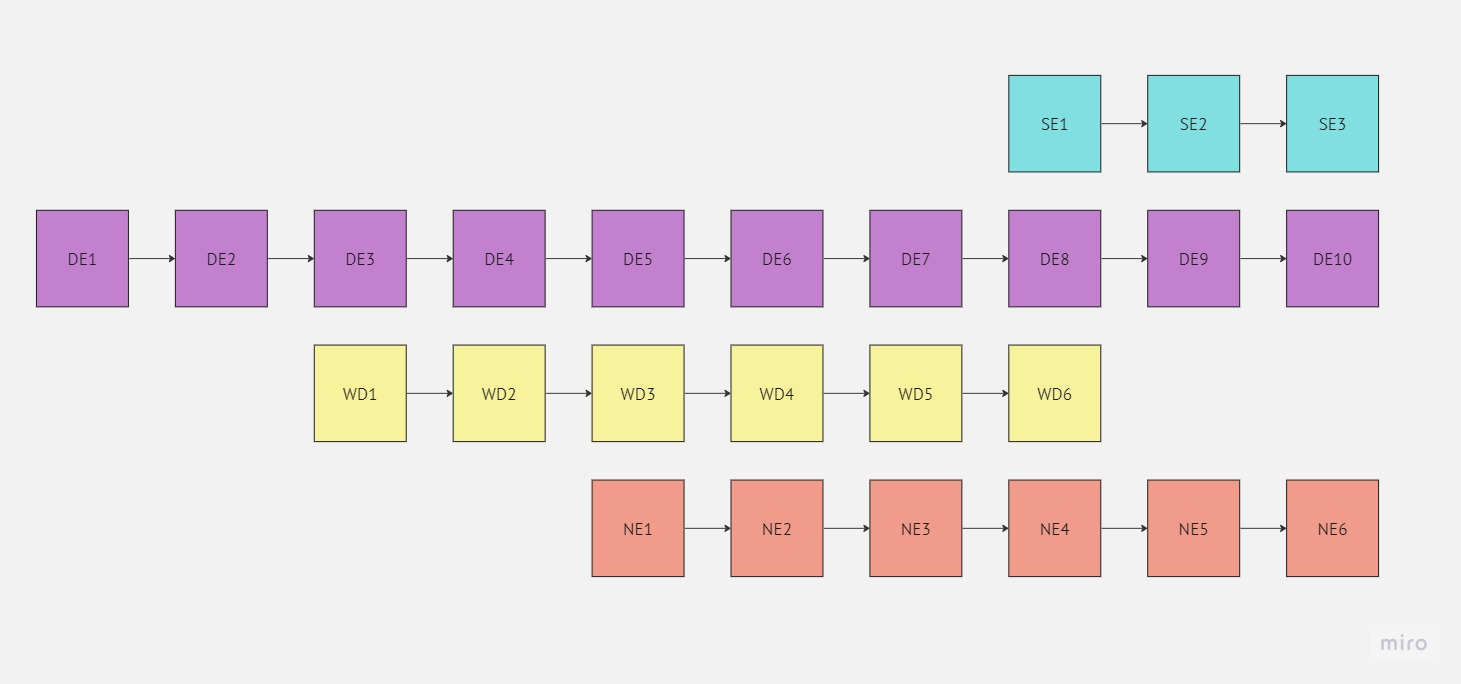
\includegraphics[width=\linewidth]{img/flowchart-development.jpg}
	\caption{Stappenplan voor de ontwikkeling van het component voor lectoren.}
	\label{img:stappenplan-leerkrachten}
\end{figure}

\begin{center}
	\begin{table}
		\begin{tabular}{ | m{2cm} | m{12cm} | } 
			\hline
			WD1 & Flask-skelet aanmaken \\
			WD2 & Formulier voor GPT-3 API-sleutel invoer maken + sessie \\
			WD3 & Formulier voor gepersonaliseerde opties van website aanmaken + sessie \\
			WD4 & Webpagina's aanmaken in HTML \& CSS \\
			WD5 & Invoerformulier maken voor PDF- en tekstupload \\
			WD6 & Invoerformulier maken voor het genereren van een gepersonaliseerde vereenvoudiging van een wetenschappelijk artikel \\
			\hline
		\end{tabular}
		\caption{Taken van de webontwikkelaar bij het uitwerken van het lerarencomponent.}
		\label{table:tasks-web-engineer}
	\end{table}
\end{center}

\begin{center}
	\begin{table}[H]
		\begin{tabular}{ | m{2cm} | m{12cm} | } 
			\hline
			NE1 & Spacy word embeddings laden \&PoS-tagging en lemmatization implementeren \\
			NE2 & Dictionary implementen voor het bijhouden van de PoS-tag per dictionary \\
			NE3 & Jupyter notebook om gepersonaliseerde prompts en aangepaste hyperparameters uit te testen voor de GPT-3 API \\
			NE4 & Jupyter notebook gebruiken om tekstvereenvoudigingsfuncties met GPT-3 API uit te testen. \\
			NE5 & Optioneel: Extra trainingsdata toevoegen aan GPT-3 model. \\
			NE6 & Code voor de voorgestelde pipeline voor ATS implementeren in Python back-end. \\
			\hline
		\end{tabular}
		\caption{Taken van de NLP Engineer bij het uitwerken van het lerarencomponent.}
		\label{table:tasks-nlp-engineer}
	\end{table}
\end{center}


\begin{center}
	\begin{table}[H]
		\begin{tabular}{|m{2cm}|m{12cm}|}
			\hline
			DE1	& Python-notebook om PDFMiner uit te testen bij willekeurige wetenschappelijke artikelen (2000 - nu) \\
			DE2 & Python-notebook opstellen om EasyOCR uit te testen bij willekeurige wetenschappelijke artikelen \\
			DE3 & Jupyter notebook om tekstdata cleaning te realiseren. De restanten van de PDF-extractie moeten weg. \\
			DE4 & Jupyter notebook om look-up methode voor synoniemen te realiseren. \\
			DE5 & Code in back-end implementeren voor PDF-upload via in-memory PDF read. \\
			DE6 & Python-notebook om Pandoc PDF \& Word-document te genereren. \\
			DE7 & Uittesten van YAML-header in Markdown-bestand voor een document op maat. \\
			DE8 & Uittesten van uitschrijven tekstinhoud naar Markdown-bestand \\
			DE9 & Implementatie code van Pandoc in Flask-framework \\
			DE10 & Code in back-end implementeren voor zippen \& doorsturen naar eindgebruiker. \\
			\hline
		\end{tabular}
			\caption{Taken van data engineer bij het uitwerken van het lerarencomponent.}
			\label{table:tasks-data-engineer}
	\end{table}
\end{center}

\begin{center}
	\begin{table}
		\begin{tabular}{|m{2cm}|m{12cm}|}
			\hline
			SE1 & Dockerfile en bijhorende requirementsfile aanmaken \\
			SE2 & Opzet in Docker realiseren \\
			SE3 & Powershell en Bash-script realiseren \\
			\hline
		\end{tabular}
		\caption{Taken van de system engineer bij het uitwerken van het lerarencomponent.}
		\label{table:tasks-system-engineer}
	\end{table}
\end{center}


\subsection{Tool voor scholieren}

De taken van de NLP engineer blijven vrijwel identie, daarmee verwijst dit onderdeel terug naar tabel \ref{table:tasks-nlp-engineer}. Daarnaast vallen de taken van de systeemingenieur in dezelfde lijn als die bij het lerarencomponent, daarmee verwijst dit component opnieuw naar de taken verwezen in tabel \ref{table:tasks-system-engineer}. De bijhorende flowchart wordt weergegeven in figuur \ref{img:stappenplan-scholars}.

\medspace

\begin{figure}[H]
	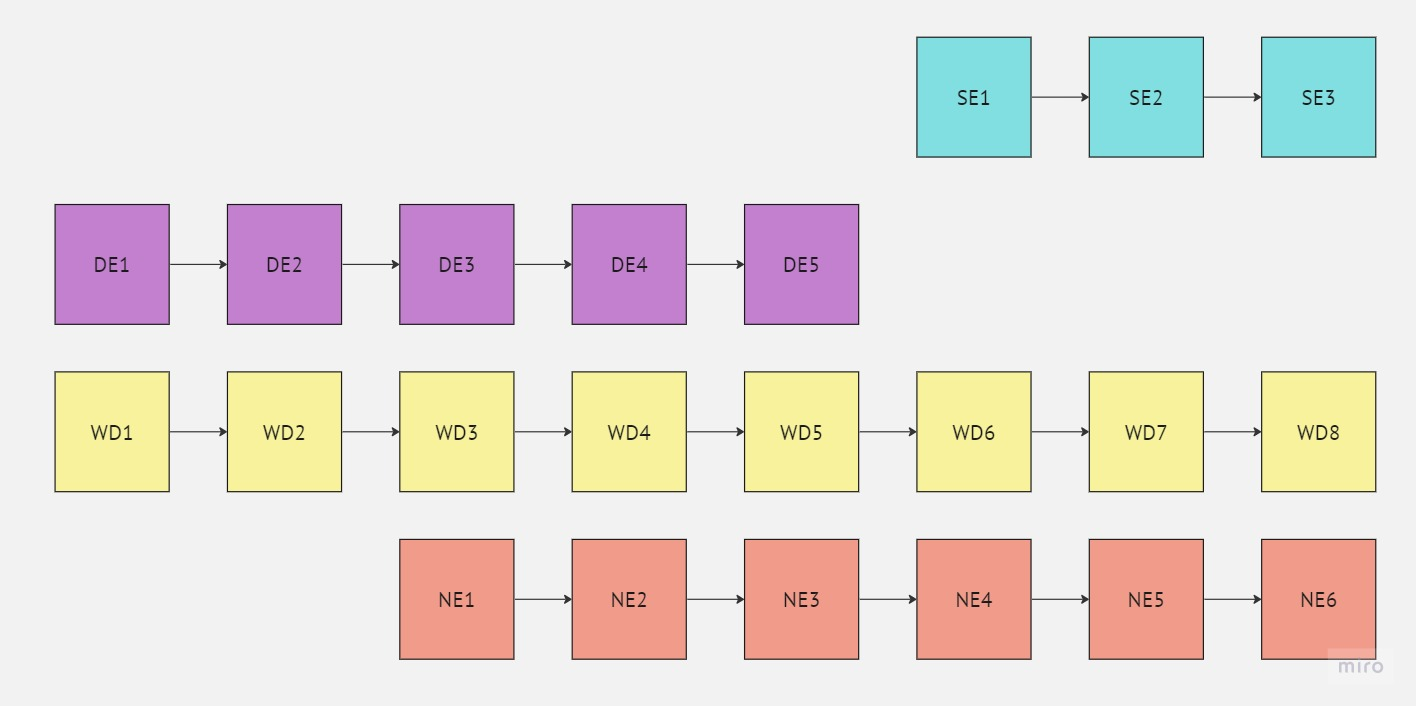
\includegraphics[width=\linewidth]{img/flowchart-development-scholars.jpg}
	\caption{Stappenplan voor de ontwikkeling van het component voor scholieren.}
	\label{img:stappenplan-scholars}
\end{figure}

\begin{center}
	\begin{table}
		\begin{tabular}{ | m{2cm} | m{12cm} | } 
			\hline
			WD1 & Flask-skelet aanmaken \\
			WD2 & Formulier voor GPT-3 API-sleutel invoer maken + sessie \\
			WD3 & Formulier voor gepersonaliseerde opties van website aanmaken + sessie \\
			WD4 & Webpagina's aanmaken in HTML \& CSS \\
			WD5 & Invoerformulier maken voor PDF- en tekstupload \\
			WD6 & JavaScript-functies schrijven voor het weergeven van grammaticale structuren, bijvoeglijke en zelfstandige naamwoorden. \\
			WD7 & JavaScript functies schrijven voor dynamische tekstaanpassing met placeholder-tekst \\
			WD8 & API-calls schrijven voor de functies: look-up, lexicale vereenvoudiging, formaatwijzigingen en ten slotte prompt-gedreven tekstvereenvoudiging \\
			\hline
		\end{tabular}
		\caption{Taken van NLP engineer bij het uitwerken van het scholierencomponent.}
		\label{table:tasks-nlp-engineer-scholars}
	\end{table}
\end{center}

\begin{center}
	\begin{table}[H]
		\begin{tabular}{|m{2cm}|m{12cm}|}
			\hline
			DE1	& Python-notebook om PDFMiner uit te testen bij willekeurige wetenschappelijke artikelen (2000 - nu) \\
			DE2 & Python-notebook opstellen om EasyOCR uit te testen bij willekeurige wetenschappelijke artikelen \\
			DE3 & Jupyter notebook om tekstdata cleaning te realiseren. De restanten van de PDF-extractie moeten weg. \\
			DE4 & Jupyter notebook om look-up methode voor synoniemen te realiseren. \\
			DE5 & Code in back-end implementeren voor PDF-upload via in-memory PDF read. \\
			\hline
		\end{tabular}
		\caption{Taken van data engineer bij het uitwerken van het scholierencomponent.}
		\label{table:tasks-data-engineer-scholars}
	\end{table}
\end{center}

Allereerst wordt de pagina voor de weergaven van het wetenschappelijk artikel opgebouwd in HTML, CSS en Jinja. De iteratiestructuur uit het lerarencomponent, verwezen in \ref{} kan overgenomen worden om code te herbruiken. De algemene weergave van dit component oogt in dezelfde lijn als dat van de uitgeteste chatbots, maar afgetoetst op de benodigde kenmerken verwezen in tabel \ref{table:dyslexia-necessaries}. Figuur \ref{img:proto-homescreen-scholieren} presenteert een voorbeeldweergave van het scholierencomponent. De front-end beschikt al over de PoS-tags en daarmee kan de gebruiker zelf kleuren selecteren om specifieke woorden te markeren. Figuur \ref{img:proto-pos-tagging-scholieren} geeft een voorbeeldweergave van deze functionaliteit. De werkwoorden worden hieronder afgebeeld in het donkerblauw, in tegenstelling tot bijvoeglijke naamwoorden die een donkergroene kleur hebben.

\begin{center}
	\begin{figure}[H]
		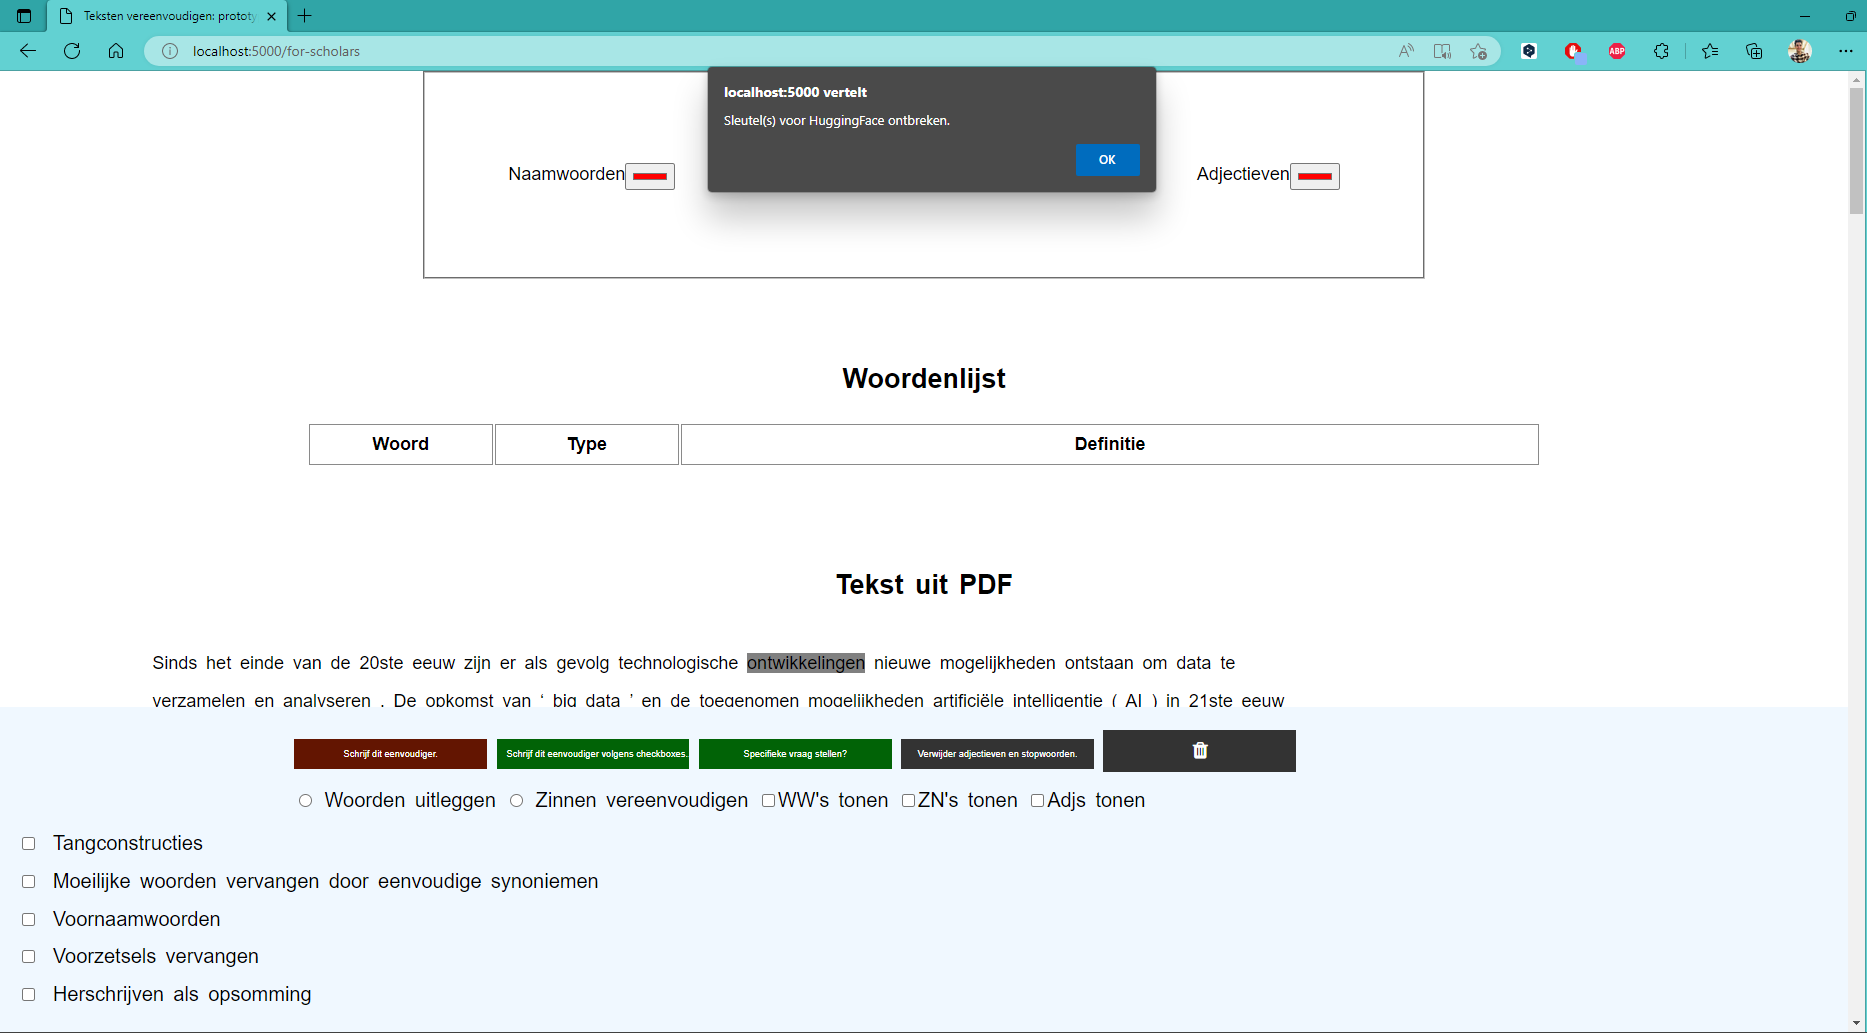
\includegraphics[width=\linewidth]{img/proto-melding.png}
		\caption{Een voorbeeldweergave van het scholierencomponent.}
		\label{img:proto-homescreen-scholieren}
	\end{figure}
\end{center}

\begin{center}
	\begin{figure}[H]
		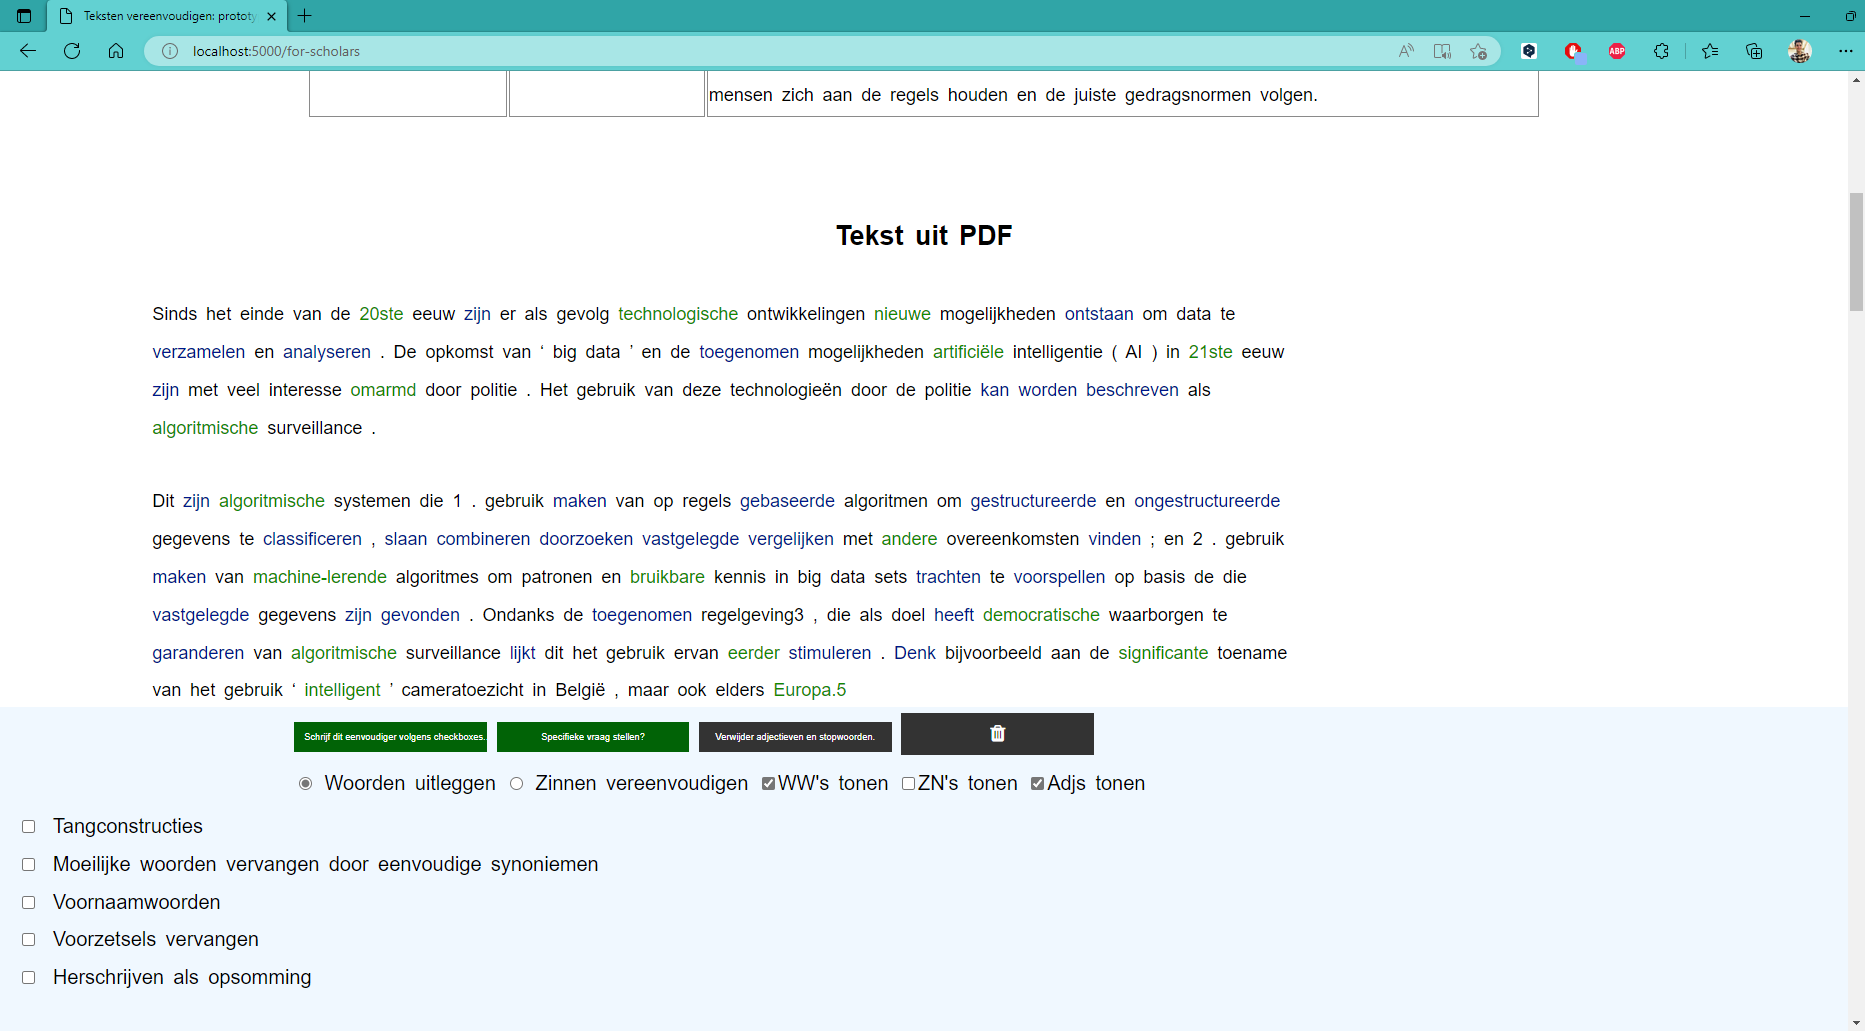
\includegraphics[width=\linewidth]{img/proto-pos-tagging.png}
		\caption{Een voorbeeldweergave van de toepassing van PoS-tagging bij het scholierencomponent.}
		\label{img:proto-pos-tagging-scholieren}
	\end{figure}
\end{center}

Scholieren kunnen weergegeven tekst markeren met hun cursor om deze vervolgens te vereenvoudigen op maat van hun noden. Zo kan de webpagina waarbij een scholier een opsomming wilt van een tekst er uit zien zoals in figuren \ref{img:proto-scholieren-step-1} en \ref{img:proto-scholieren-step-3}. Allereerst wordt de gemarkeerde tekst en de meegegeven gepersonaliseerde opties via JavaScript opgeslaan en doorgegeven aan de back-end. Vervolgens handelt de back-end de API-call naar GPT uit met een prompt waarin dynamisch de personalisatieopties aan worden geconcateneerd. Als de tekst doorlopend is, dan verwerkt JavaScript dit resultaat als een p-tag. Als de scholier eerder koos voor een opsomming, dan wordt er in de prompt ook expliciet een formaat verwacht. Op basis van dit formaat wordt er een ul-tag aangemaakt waarin de array van zinnen wordt geitereerd met een li-tag.

\begin{center}
	\begin{figure}[H]
		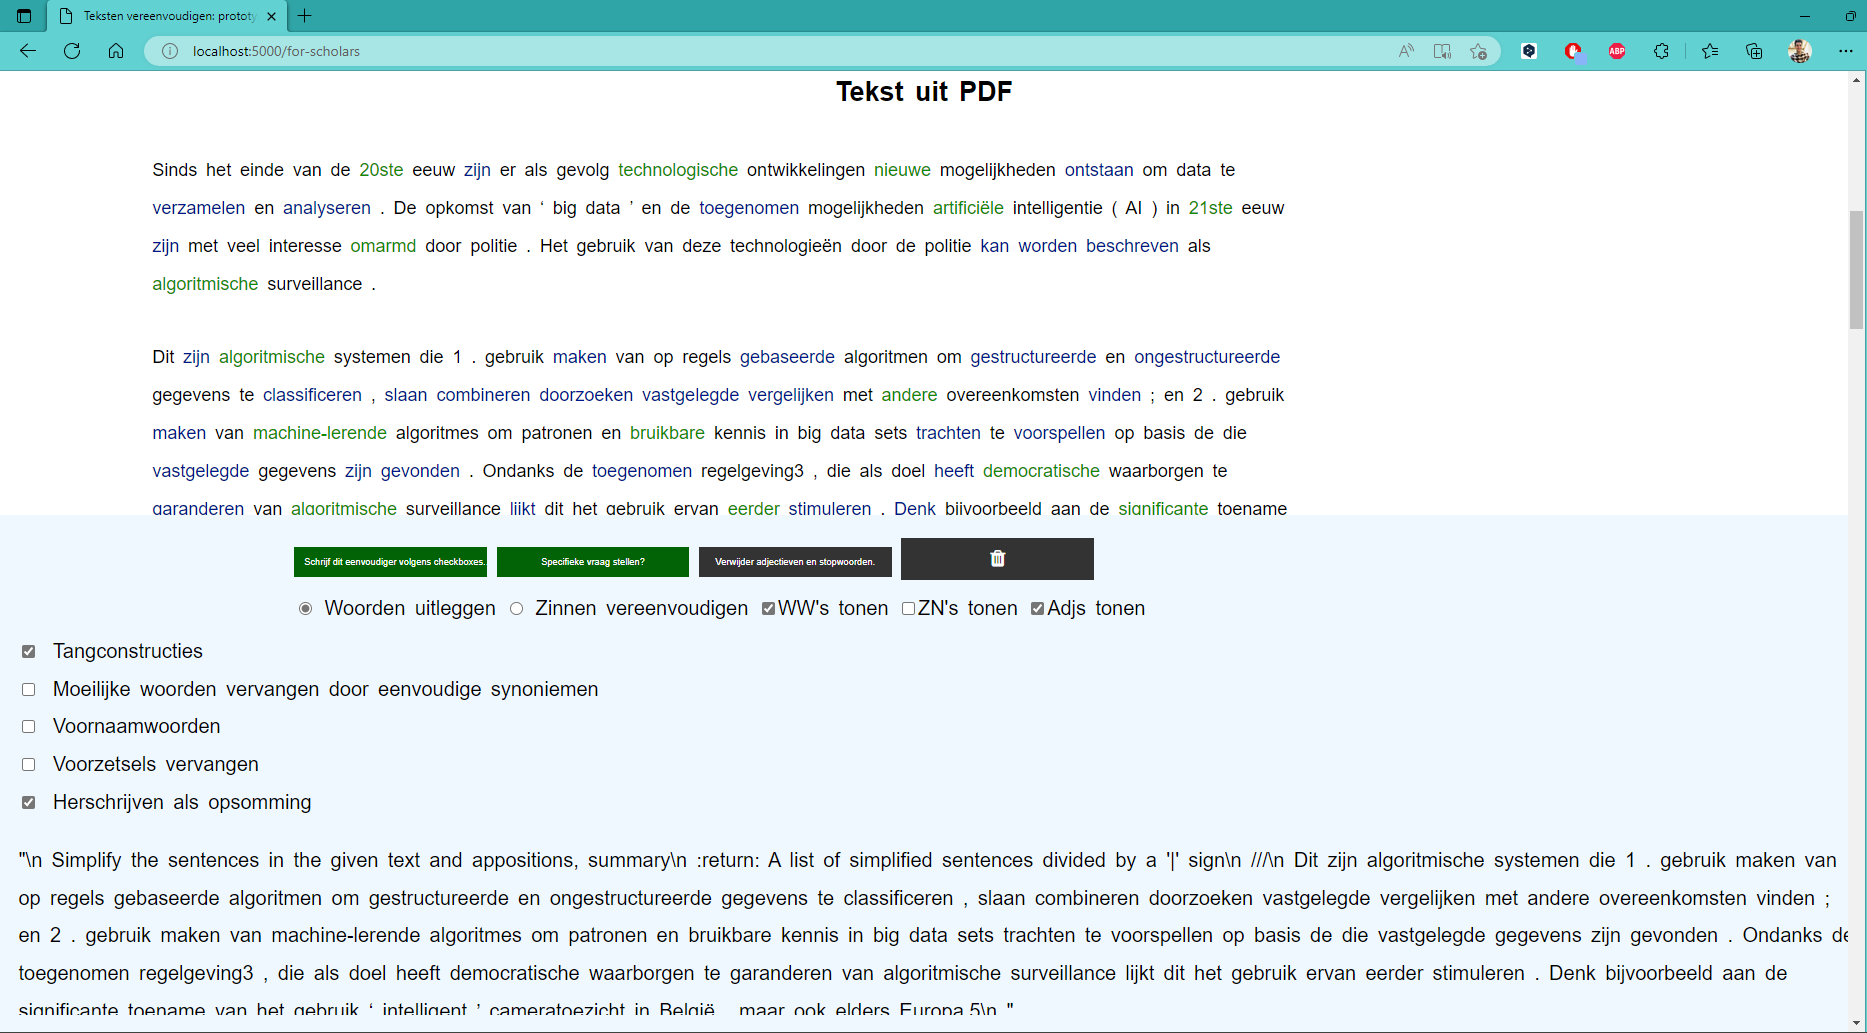
\includegraphics[width=\linewidth]{img/proto-opsomming-1.png}
		\caption{Stap 1 van een gepersonaliseerde tekstvereenvoudiging in het scholierencomponent.}
		\label{img:proto-scholieren-step-1}
	\end{figure}
\end{center}

\begin{center}
	\begin{figure}[H]
		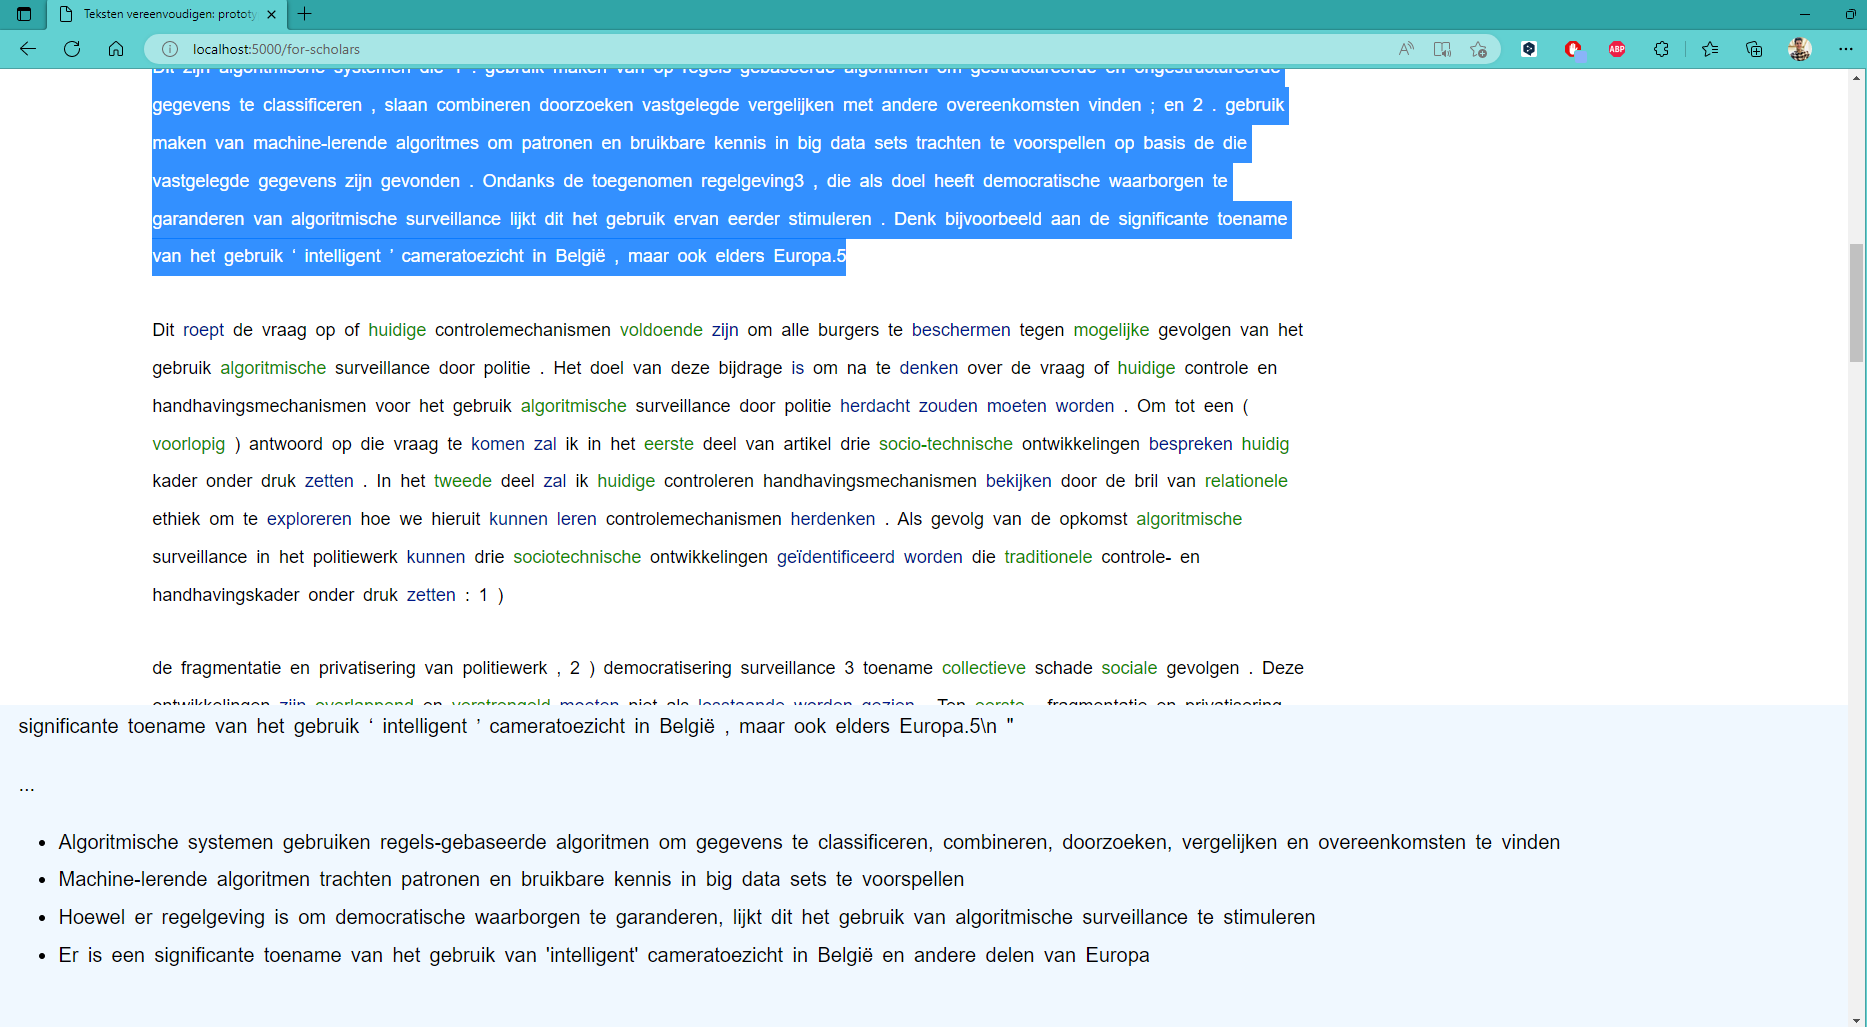
\includegraphics[width=\linewidth]{img/proto-opsomming-3.png}
		\caption{Stap 3 van een gepersonaliseerde tekstvereenvoudiging in het scholierencomponent.}
		\label{img:proto-scholieren-step-3}
	\end{figure}
\end{center}

Scholieren kunnen zelf vragen stellen door de tekst te markeren en vervolgens op de verwante knop te drukken. Een JavaScript-call stuurt dan de prompt en de tekst naar de Flask back-end. Die verwerkt de aanvraag met de functie in de zelfgemaakte GPT-klasse. Om het systeem robuust te maken, wordt er aan de prompt een extra veiligheidsmaatregel toegevoegd, namelijk 'op basis van deze tekst ///'. Om transparantie van het model te garanderen, geeft de back-end ook de prompt mee aan de front-end. Deze twee stappen worden afgebeeld in figuren \ref{img:step-1-proto-vraagstelling} en \ref{img:step-2-proto-vraagstelling}.

\begin{center}
	\begin{figure}
		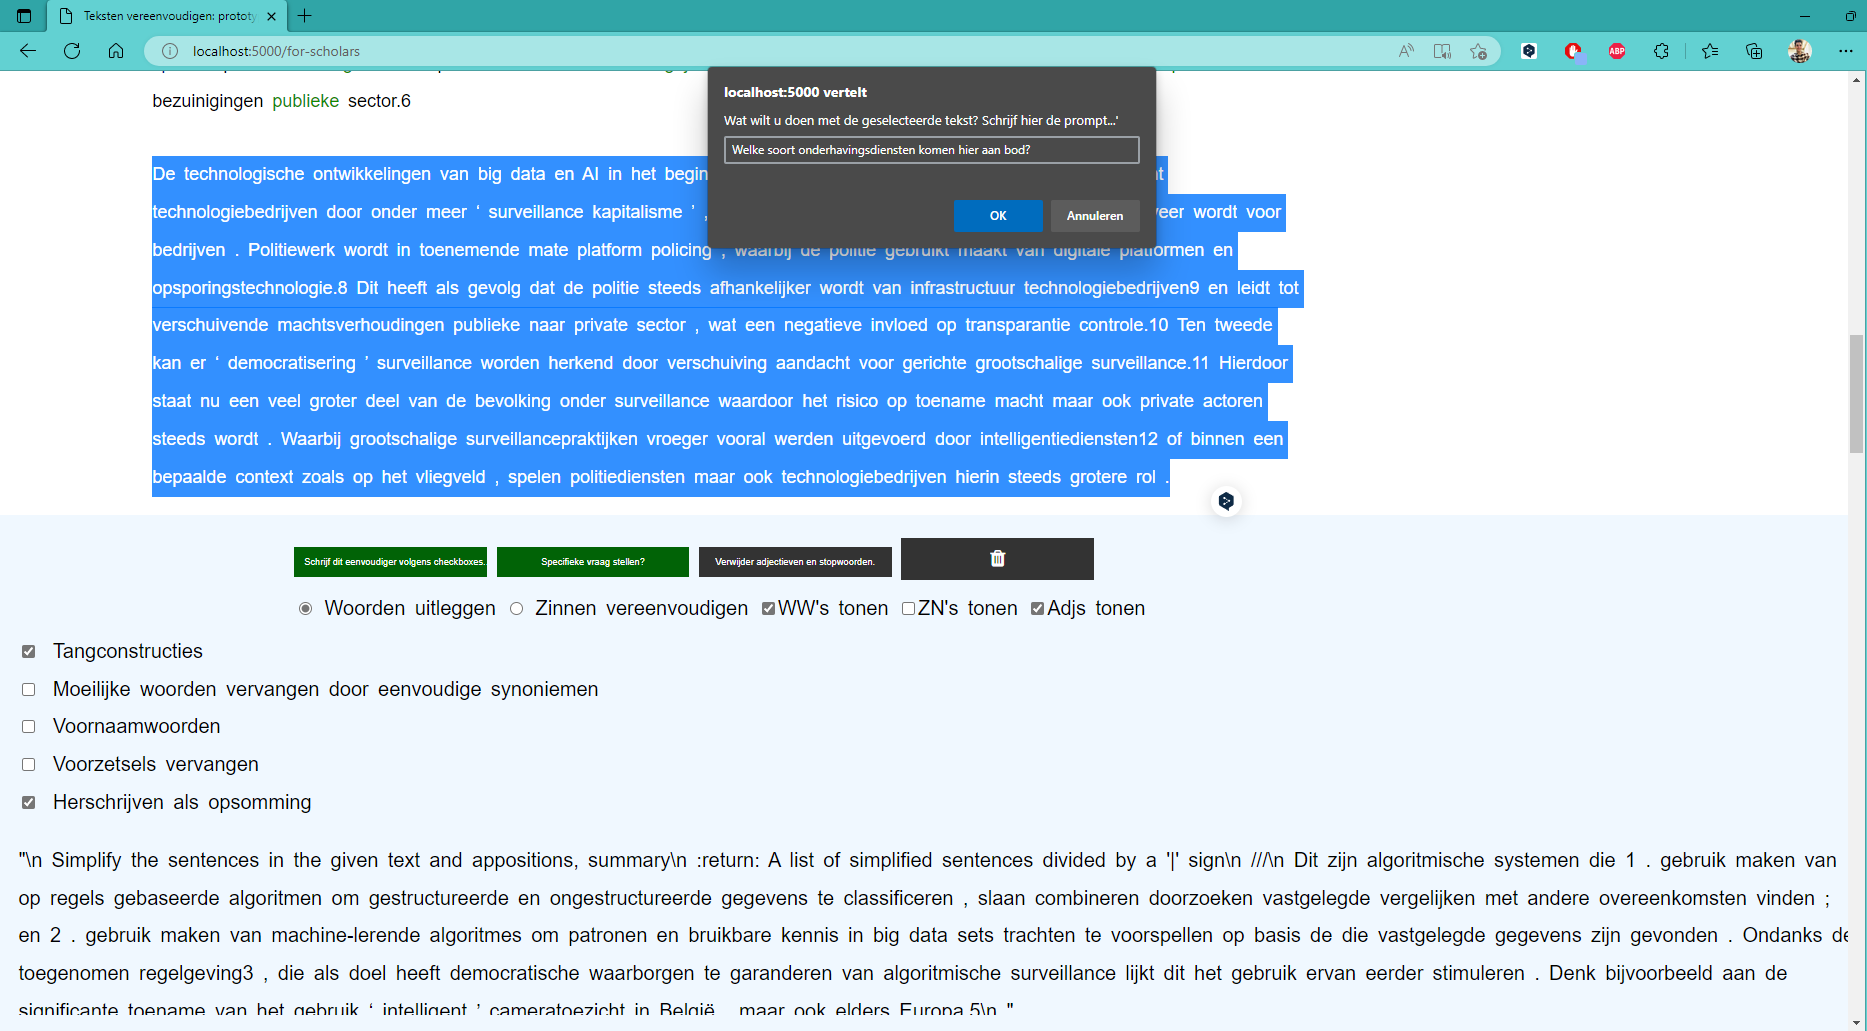
\includegraphics[width=\linewidth]{img/proto-vraagstelling-1.png}
		\caption{Stap 1 bij het stellen van een specifieke vraag bij gemarkeerde tekst.}
		\label{img:step-1-proto-vraagstelling}
	\end{figure}
\end{center}

\begin{center}
	\begin{figure}
		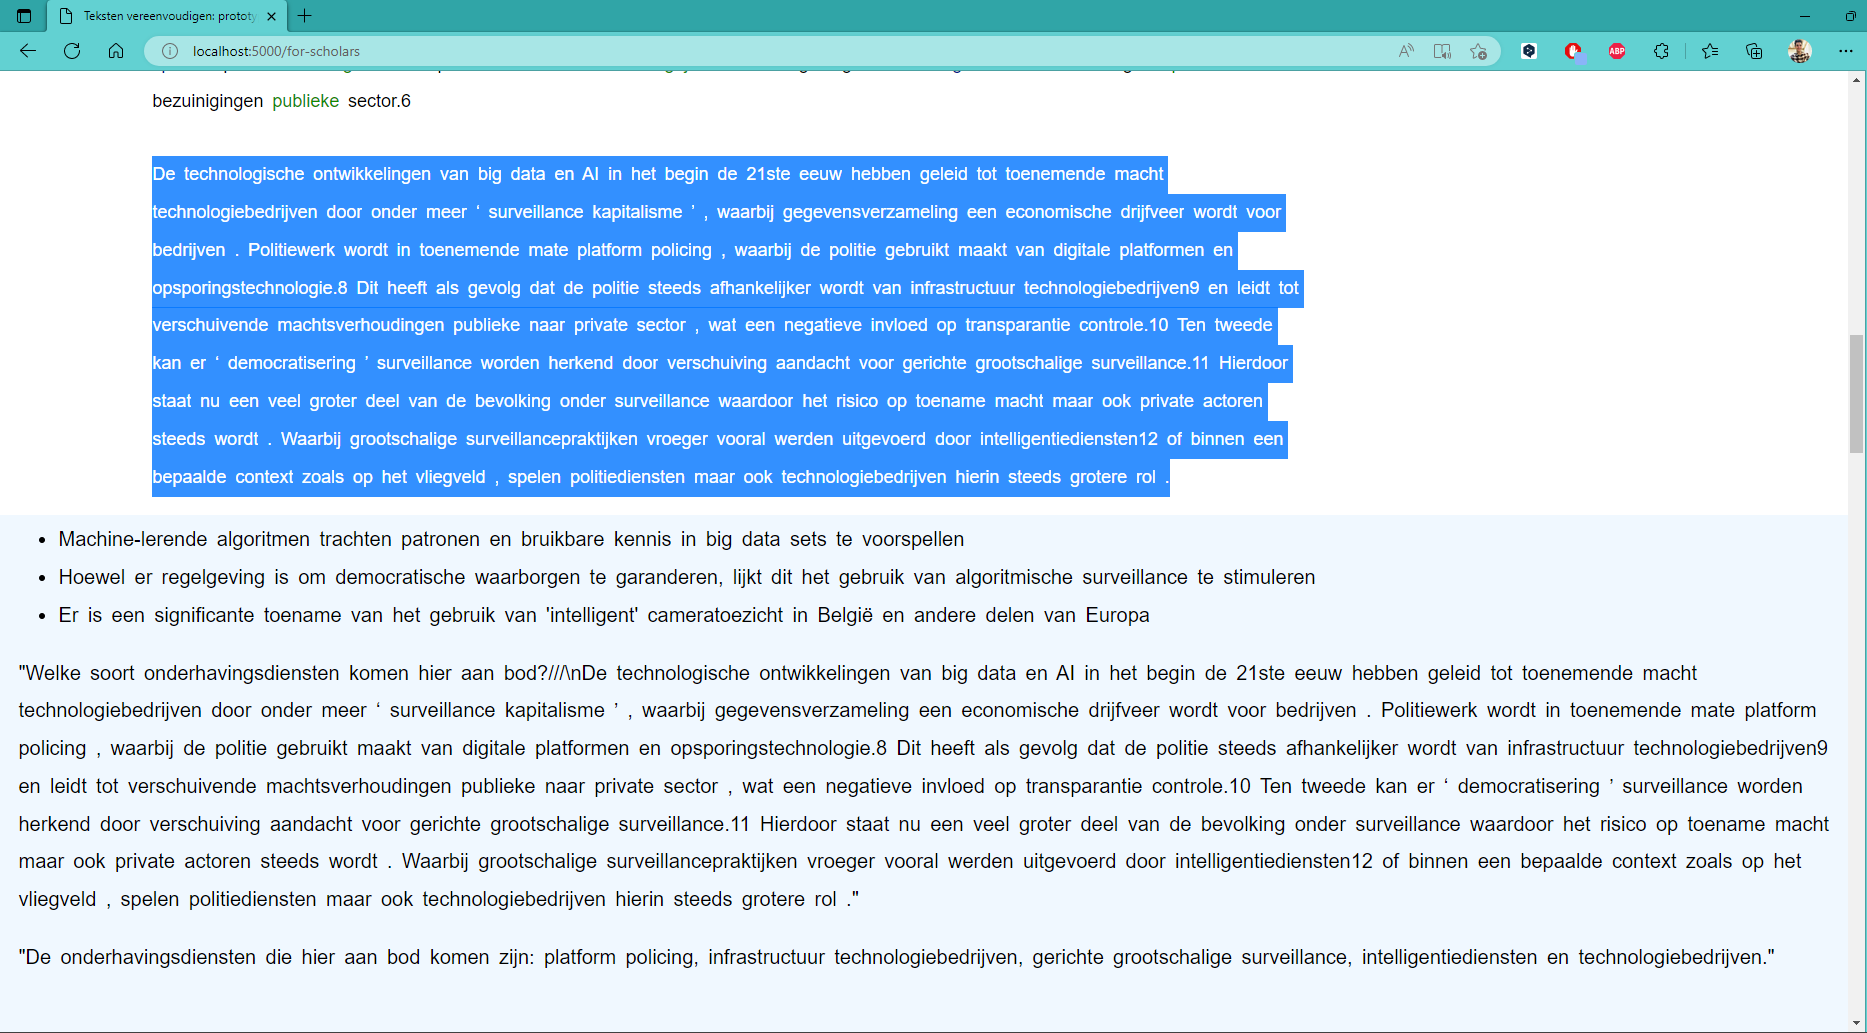
\includegraphics[width=\linewidth]{img/proto-vraagstelling-2.png}
		\caption{Stap 2 bij het stellen van een specifieke vraag bij gemarkeerde tekst.}
		\label{img:step-2-proto-vraagstelling}
	\end{figure}
\end{center}

\medspace

Ten slotte maakt het prototype gebruik van Docker voor de lokale opzet. Een scriptbestand, in Powershell of Bash, vereenvoudigt de opstart van deze webapplicatie, in tegenstelling tot de opstart per terminal. Alvorens installeert Docker met behulp van de voorafgegeven instructies de nodige Python-bibliotheken met het Pipreq-commando. Omdat het prototype gebruik maakt van de API's van de taalmodellen, hoeft het prototype geen gebruik te maken van een aparte container voor het taalmodel.

% Ontwikkelaars moeten rekening houden met het gebrek aan structuur bij het ophalen van tekstinhoud uit een PDF-bestand.